\documentclass[11pt]{article}

\usepackage[margin=1in]{geometry}
\usepackage{graphicx}
\graphicspath{{figures/}}
\usepackage{amsmath,amssymb}
\usepackage{bm}
\usepackage{booktabs}
\usepackage{subcaption}
\usepackage[numbers,sort&compress]{natbib}
\usepackage{xcolor}
\usepackage{caption}
\captionsetup{font=small,labelfont=bf}
\usepackage[colorlinks=true,linkcolor=blue,citecolor=blue,urlcolor=blue]{hyperref}

% --- convenience macros for consistent notation across the paper ---
\newcommand{\xstate}{\bm{x}}          % physical state
\newcommand{\yobs}{\bm{y}}            % observation
\newcommand{\Hop}{H}                  % observation operator
\newcommand{\Hinv}{H^{-1}_{\theta}}  % learned inverse observation operator
\newcommand{\Mop}{\mathcal{M}}        % forward model / integrator
\newcommand{\Jb}{J_{\mathrm{b}}}     % background cost
\newcommand{\Jo}{J_{\mathrm{o}}}     % observation cost
\newcommand{\Bcov}{\bm{B}}           % background covariance
\newcommand{\Rcov}{\bm{R}}           % observation covariance
\newcommand{\sigb}{\sigma_{\mathrm{b}}}
\newcommand{\sigobs}{\sigma_{\mathrm{obs}}}
\newcommand{\rmse}{\mathrm{RMSE}}

\title{\textbf{Full Four-Dimensional Variational Data Assimilation with a\\
Learned Inverse Observation Operator under Observation Noise}}

\author{
  Eric Xu \and Javier Sanchez \and Jiayang Wu \and Wilson Xie \and Edmund Xu \\[4pt]
  \small AM 170B --- Applied Mathematics Capstone
}

\date{May 2026}

\begin{document}

\maketitle

\begin{abstract}
Variational data assimilation (DA) estimates the initial state of a dynamical system by fitting a
model trajectory to sparse observations, but when the observation operator is non-invertible the
resulting cost function is riddled with poor local minima. Frerix et al. (2021) addressed this by
training a learned inverse observation operator---a convolutional neural network (CNN) that lifts
observations back into physical space---and using it to initialize and reshape the assimilation
objective. We reimplement their approach in PyTorch and extend it in three ways: we replace their
simplified observation-misfit objective with the full four-dimensional variational (4D-Var) cost,
adding an explicit background term and observation-error covariance; we corrupt every experiment
with additive Gaussian observation noise at three magnitudes; and we wrap the solver in an
operational sliding-window (cycling) scheme for long-horizon assimilation. We evaluate on two
systems: the one-dimensional (1D) Lorenz-96 model and two-dimensional (2D) Kolmogorov flow, an
incompressible Navier--Stokes system. Across all noise levels, learned-inverse initialization
combined with hybrid (physics-space then observation-space) optimization yields the lowest analysis
root-mean-square error (RMSE), and sliding-window cycling stabilizes assimilation over horizons
where single-window 4D-Var degrades. We also report honest negative results, including a background
weight that tuned only marginally and an unexpected optimal-variance ordering.
\end{abstract}

\section{Introduction}

Numerical weather prediction (NWP) launches a forecast by integrating a numerical
model of the atmosphere forward from an estimate of its current state. Because the
atmosphere is observed only incompletely, indirectly, and noisily, producing that
initial estimate is itself an inverse problem: given a forecast model and a stream of
imperfect measurements distributed in space and time, recover the system state well
enough to forecast from it. This is the task of data assimilation (DA), and it is the
component of an operational NWP system that most directly limits forecast skill
\citep{kalnay2003atmospheric}. The flagship variational method is
four-dimensional variational data assimilation (4D-Var)
\citep{ledimet1986variational, courtier1994strategy}, which estimates the initial
condition $\xstate_0$ of an assimilation window by minimizing a cost that balances a
prior (``background'') estimate against the misfit between the model trajectory and the
observations spread across that window.

DA is hard precisely because the systems of interest are chaotic: small errors in the
analysis (the assimilated initial state) grow exponentially, so the analysis must be
accurate and the optimization landscape is treacherous. The Lorenz-96 model
\citep{lorenz1996predictability} is the canonical low-order testbed for exactly this
difficulty, and it is the primary one-dimensional (1D) system we study here. In our
configuration (grid size 40, forcing $F=8$), trajectories started $10^{-6}$ apart
separate at a fitted exponential rate $\lambda = 2.263\,/\mathrm{MTU}$, corresponding to
a Lyapunov time $T_L = 1/\lambda = 0.442$ model time unit (MTU); this is somewhat
shorter than the $\sim$0.6 MTU expected from the original study, a known artifact of our
fixed-step integrator that we report honestly. Because errors saturate within roughly a
Lyapunov time, an inaccurate analysis cannot be rescued downstream, and this is the
regime in which a better treatment of the observations is supposed to help.

\paragraph{The learned inverse-observation idea.}
\citet{frerix2021invobs} study the variational problem of recovering an initial state
$\xstate_0$ whose model trajectory $\Mop^t(\xstate_0)$ fits a sequence of observations.
The observation operator $\Hop$ in their setting (and ours) is a sparse spatial
subsampling: it keeps every fourth grid point for Lorenz-96 (10 of 40 points observed)
and every sixteenth point in each direction for two-dimensional (2D) Kolmogorov flow (a
$4\times4=16$ of 4096 points observed). Because $\Hop$ is many-to-one and highly lossy,
the standard observation-space objective
$\lVert \Hop\,\Mop^t(\xstate_0) - \yobs_t\rVert^2$ is strongly non-convex and riddled
with bad local minima, so a poorly initialized gradient-based optimizer gets trapped.
Their contribution is to train a convolutional neural network (CNN) that acts as a
learned inverse observation operator $\Hinv$, mapping an observation sequence back into
physics (state) space. They use it in two complementary ways: as a better
\emph{initialization} (lift the observations to a physics-space first guess
$\Hinv(Y)$ instead of a naive interpolation or average), and as a \emph{reformulation of
the loss} (replace the observation-space misfit with a physics-space misfit
$\sum_t \lVert \Mop^t(\xstate_0) - [\Hinv(Y)]_t\rVert^2$, which removes the lossy $\Hop$
from inside the objective and is therefore much closer to convex). They further propose
an optional \emph{hybrid} schedule: run the smoother physics-space optimization first as
a warm start, then refine against the true observations in observation space. Crucially
for our work, the original study assimilates \emph{clean} observations and uses a
\emph{simplified} objective (the observation-misfit term only, with no background term
and no explicit observation-error covariance), and its reference implementation is in
JAX/Flax.

\paragraph{Our contribution.}
This capstone tests whether the learned inverse-observation idea survives a more
operationally realistic setting, through four changes. (i)~\emph{Full 4D-Var cost.}
We replace the paper's observation-misfit-only objective with the complete 4D-Var cost
$J(\xstate_0) = \Jb + \Jo$,
\[
  J(\xstate_0) = \tfrac12 (\xstate_0-\xstate_b)^\top \Bcov^{-1} (\xstate_0-\xstate_b)
  + \tfrac12 \sum_{t} \big(\Hop \Mop^t(\xstate_0) - \yobs_t\big)^\top \Rcov^{-1}
    \big(\Hop \Mop^t(\xstate_0)-\yobs_t\big),
\]
with background covariance $\Bcov = \sigb^2 \bm{C}$ ($\bm{C}$ the system's spatial
correlation) and observation-error covariance $\Rcov = \sigobs^2 \bm{I}$. The background
term pulls the analysis toward a prior $\xstate_b$ and is what makes the problem
well-posed when observations are sparse; $\sigb$ is the background-error standard
deviation we tune and $\sigobs$ the observation-error standard deviation.
(ii)~\emph{Observation noise.} Every experiment adds independent Gaussian observation
noise with $\sigobs \in \{0.1, 0.5, 1.0\}$ (the paper used clean observations), which
both stress-tests robustness and probes a deliberate mismatch, since the inverter is
trained at one noise level and evaluated at others. (iii)~\emph{Sliding-window cycling.}
We add an operational sliding-window (cycling) 4D-Var extension in which short
assimilation windows are advanced through time and each cycle's analysis is propagated
forward to form the background for the next window---the way 4D-Var is actually run
operationally, in contrast to the paper's single fixed window.
(iv)~\emph{PyTorch reimplementation.} We rebuild the entire pipeline in PyTorch
\citep{paszke2019pytorch}---the dynamical-system integrators, the CNN inverter, the
correlation preconditioning, and the data-assimilation loop solved with the
limited-memory Broyden--Fletcher--Goldfarb--Shanno (L-BFGS) optimizer
\citep{liu1989limited}.

Our headline finding is that the paper's central claim broadly holds under these harder
conditions: learned-inverse-observation initialization combined with hybrid optimization
attains the lowest analysis root-mean-square error (RMSE) at every tested noise level,
and hybrid optimization dramatically rescues a cheap climatological-mean baseline that
observation-only optimization leaves stuck in a bad local minimum. We also report honest
negative results, notably that a secondary expectation about how the optimal $\sigb$
should shift did not hold, and that on the smoke-scale Kolmogorov-flow runs the cycling
extension does not yet show a decisive advantage.

\paragraph{Roadmap.}
The remainder of the paper is organized as follows. Section~2 summarizes the learned
inverse-observation approach of \citet{frerix2021invobs} and states precisely how we
extend it. Section~3 describes the models and methods: the Lorenz-96 and Kolmogorov-flow
dynamical systems and their integrators, the observation-noise model, the full 4D-Var
cost and its physics-space hybrid companion, the learned inverse observation operator,
the decorrelation preconditioning, and the sliding-window cycling scheme. Section~4
presents results, first for Lorenz-96 (integrator diagnostics, inverter training,
baseline initialization, the tuned-$\sigb$ full 4D-Var sweep, and the sliding-window
experiments) and then for two-dimensional Kolmogorov flow. Section~5 discusses
limitations and caveats, separating what reproduces the paper from what our extensions
add, and concludes.

\section{Background: The Learned Inverse-Observation Approach and Our Extensions}
\label{sec:background}

\subsection{The Method We Extend}

DA estimates the state of a dynamical system from a forecast model together with a stream of incomplete, indirect, and noisy observations, so that a forecast can be launched from the resulting analysis~\citep{kalnay2003atmospheric}. The flagship operational method is 4D-Var, which recovers the initial condition $\xstate_0$ of a forecast window by minimizing a cost that balances a prior estimate against the misfit between the model trajectory and observations distributed in time~\citep{ledimet1986variational,courtier1994strategy}. The difficulty is intrinsic to the chaotic systems that DA targets: in the Lorenz-96 testbed~\citep{lorenz1996predictability} small errors grow exponentially, so the analysis must be accurate and the optimization landscape is treacherous.

\citet{frerix2021invobs} study the variational problem of recovering an initial state $\xstate_0$ whose model trajectory $\Mop^t(\xstate_0)$ fits a sequence of observations. The observation operator $\Hop$ is a sparse spatial subsampling: it retains every fourth grid point for Lorenz-96 (10 of 40 sites observed) and every sixteenth point in each direction for 2D Kolmogorov flow (a $4\times 4 = 16$ of 4096 sites observed). Because $\Hop$ is many-to-one and highly lossy, the standard observation-space objective $\lVert \Hop\,\Mop^t(\xstate_0) - \yobs_t\rVert^2$ is strongly non-convex and riddled with bad local minima, and a gradient-based optimizer started from a poor first guess is easily trapped.

The contribution of \citet{frerix2021invobs} is to train a CNN that acts as a learned inverse observation operator $\Hinv$, mapping an observation sequence $Y$ back into physical-state space. They exploit this operator in two complementary ways. First, as a better \emph{initialization}: the observations are lifted to a physics-space first guess $\Hinv(Y)$ instead of a naive interpolation or averaging baseline. Second, as a \emph{reformulation of the loss}: the lossy observation-space misfit is replaced by a physics-space misfit
\[
\sum_t \bigl\lVert \Mop^t(\xstate_0) - [\Hinv(Y)]_t \bigr\rVert^2,
\]
which is much closer to convex because it removes $\Hop$ from inside the objective. They further propose an optional \emph{hybrid} schedule: run physics-space optimization first as a warm start, then refine against the true observations in observation space, thereby keeping the smoother physics-space basin of attraction while finishing on the genuine measurement misfit. The approach is demonstrated on two systems --- Lorenz-96 (one-dimensional) and 2D Kolmogorov flow (incompressible Navier--Stokes with Kolmogorov forcing) --- and the reference implementation is in JAX/Flax with a JAX-CFD solver for the flow~\citep{kochkov2021machine}.

Crucially for our work, the original study makes two simplifications. It assimilates \emph{clean} observations with no added measurement noise, and it minimizes an objective that contains \emph{only} the observation-misfit term: there is no background (prior) term and no explicit observation-error covariance.

\subsection{Our Extensions}

Our capstone asks whether the learned-inverse-observation idea survives a more operationally realistic setting. We make four changes, each stated precisely below.

\begin{enumerate}
  \item \textbf{Full 4D-Var cost.} We replace the observation-misfit-only objective with the complete 4D-Var cost $J(\xstate_0) = \Jb + \Jo$ that includes a background term and an explicit observation-error covariance,
  \[
  J(\xstate_0) = \tfrac12 (\xstate_0-\xstate_b)^\top \Bcov^{-1} (\xstate_0-\xstate_b)
  + \tfrac12 \sum_{t} (\Hop \Mop^t(\xstate_0) - \yobs_t)^\top \Rcov^{-1} (\Hop \Mop^t(\xstate_0)-\yobs_t),
  \]
  with background covariance $\Bcov = \sigb^2 \bm{C}$ (where $\bm{C}$ is the system's spatial correlation) and observation-error covariance $\Rcov = \sigobs^2 \bm{I}$. The background term $\Jb$ pulls the analysis toward a prior $\xstate_b$ and is what makes the problem well-posed when observations are sparse; $\sigb$ is the background-error standard deviation we tune and $\sigobs$ is the observation-error standard deviation. The physics-space hybrid companion cost analogously replaces $\Jo$ with $\tfrac{1}{2\sigma_p^2}\sum_t \lVert \Mop^t(\xstate_0) - [\Hinv(Y)]_t\rVert^2$.

  \item \textbf{Observation noise.} Every experiment now corrupts the observations with independent additive Gaussian noise, $\yobs = \Hop(\xstate) + \boldsymbol\varepsilon$ with $\boldsymbol\varepsilon \sim \mathcal{N}(0, \sigobs^2 \bm{I})$, at noise levels $\sigobs \in \{0.1, 0.5, 1.0\}$ (the original paper used clean observations). This tests robustness and also probes a deliberate mismatch, since the inverter is trained at one noise level and evaluated at others.

  \item \textbf{Sliding-window (cycling) 4D-Var.} We add an operational cycling extension in which a short assimilation window is advanced through time and each cycle's analysis is propagated forward to form the background for the next window --- the way 4D-Var is actually run operationally --- in contrast to the paper's single fixed window.

  \item \textbf{PyTorch reimplementation.} We reimplement the entire pipeline in PyTorch~\citep{paszke2019pytorch} (the original is JAX/Flax), including the dynamical-system integrators, the CNN inverter, the correlation preconditioning, and the L-BFGS-driven DA loop.
\end{enumerate}

Two implementation choices that the Methods section develops are worth flagging here so the cost above reads unambiguously. For Lorenz-96 the optimization is carried out in decorrelated coordinates $\bm{z} = \bm{C}^{-1/2}\xstate$, which turns the background term into the isotropic $\lVert\bm{z}_0-\bm{z}_b\rVert^2/(2\sigb^2)$; the measured spatial-correlation matrix $\bm{C}$ has condition number $8.72$ and climatological mean near $2.34$. For 2D Kolmogorov flow we optimize the vorticity field directly with $\Bcov = \sigb^2 \bm{I}$ (no decorrelation), because forming and factorizing a full $4096\times 4096$ spatial covariance is prohibitively expensive. We report results honestly, separating ``reproduced the paper'' from ``our extensions'' and flagging negative findings and smoke-scale caveats (small ensembles, the CPU-limited Kolmogorov runs, the noise-level mismatch above, and a short Lyapunov time induced by the fixed-step integrator) where they arise.

\section{Models and Methods}
\label{sec:methods}

This section describes the two dynamical systems we assimilate, the full
4D-Var cost we minimize, the learned inverse
observation operator and its two convolutional variants, our observation-noise
model, the correlation preconditioning, the optimizer, and the sliding-window
cycling scheme. Throughout, $\Mop^t(\xstate_0)$ denotes the model state at
outer step $t$ integrated from the initial condition $\xstate_0$, $\Hop$ is the
(sparse, subsampling) observation operator, and $\yobs_t = \Hop\Mop^t(\xstate_0)
+ \boldsymbol\varepsilon_t$ the corresponding noisy observation.

\subsection{Dynamical systems}

The first testbed is the 1D Lorenz-96 model
\citep{lorenz1996predictability}, a periodic chain of $K=40$ grid points
evolving under the ordinary differential equation (ODE)
\begin{equation}
\dot{x}_k = (x_{k+1}-x_{k-2})\,x_{k-1} - x_k + F,
\qquad x_{k+K}=x_k,
\label{eq:l96}
\end{equation}
with forcing $F=8$ and cyclic indices. We integrate
Eq.~\eqref{eq:l96} with a hand-written fixed-step fourth-order Runge--Kutta
(RK4) scheme in which each outer step $\Delta t = 0.1$ MTU is
composed of ten inner RK4 substeps of size $0.01$. The observation operator
$\Hop$ subsamples every fourth grid point, so the $40$-dimensional state is
observed at only $10$ sites.

To check that this fixed-step integrator is faithful at the short horizons
relevant to assimilation, we compared it against an adaptive Dormand--Prince
(dopri5) solver \citep{dormand1980family}. Starting from identical attractor
states, the $L^2$ trajectory divergence stays near machine precision while
$t \ll T_L$ and first reaches the order-one (state-norm) scale at a median
$t^{\star}=7.70$ MTU (range $[6.50,8.30]$ over five warmed-up states; $6.30$ MTU
for a single trajectory), saturating near $28.5$ once the trajectories fully
decorrelate by $t\approx 19.9$ MTU. A direct two-trajectory separation fit
(initial separation $10^{-6}$, fitted over $t\in[0.5,5.0]$ MTU) gives a leading
exponent $\lambda = 2.263\,\mathrm{MTU}^{-1}$ and a Lyapunov time
$T_L = 1/\lambda = 0.442$ MTU. This is shorter than the value of $\sim 0.6$ MTU
expected from the literature, a known consequence of the coarse fixed-step
integrator that we report honestly; our single-window experiments use a window
of $T=10$ outer steps ($1.0$ MTU), comfortably inside $t^{\star}$, so this
integrator choice does not contaminate the assimilation results.

The second testbed is 2D Kolmogorov flow: the vorticity form
of the incompressible Navier--Stokes equations (a partial differential
equation, PDE) on the periodic domain $[0,2\pi]^2$ with sinusoidal Kolmogorov
forcing at wavenumber $k=4$, viscosity $\nu=10^{-2}$, and linear (Rayleigh)
drag $\alpha=0.1$, following the solver design of \citet{kochkov2021machine}.
The state is a single vorticity field $\omega$ on a $64\times 64$ grid
($4096$ degrees of freedom), advanced with a pseudo-spectral RK4 solver at outer
step $0.18$ composed of $25$ inner substeps. Here $\Hop$ subsamples every
sixteenth point in each direction, giving a $4\times 4$ observation grid
($16$ of $4096$ points observed). Warmed-up initial conditions are produced by
integrating a spectrally filtered random field forward $100$ outer steps; a
warmup diagnostic confirms the flow reaches a statistically stationary
turbulent regime, with the enstrophy $\tfrac12\langle\omega^2\rangle$ rising
from $0.50$ at the smooth cold start to $\approx 9.8$ near the warmup horizon
(last-$20$-step relative drift $\approx 10.8\%$, i.e.\ approximately
quasi-stationary) and the training-trajectory vorticity spanning roughly
$[-12.3,14.1]$.

\subsection{Observation-noise model}

Departing from the original study, which assimilated clean observations, every
experiment here corrupts the observations with independent additive Gaussian
noise,
\begin{equation}
\yobs = \Hop(\xstate) + \boldsymbol\varepsilon,
\qquad
\boldsymbol\varepsilon \sim \mathcal{N}\!\left(\bm{0},\,\sigobs^2\bm{I}\right),
\label{eq:noise}
\end{equation}
applied independently at each observed site and time, so that the
observation-error covariance is $\Rcov = \sigobs^2\bm{I}$. For the Lorenz-96
single-window experiments we use $\sigobs \in \{0.1, 0.5, 1.0\}$, spanning a
range from a sharp, nearly-clean perturbation to a level comparable to the
Lorenz-96 state amplitude; Figure~\ref{fig:noisedist} plots the three
corresponding probability density functions. The sliding-window runs use
$\sigobs \in \{0.0, 0.5\}$ for Lorenz-96 and $\{0.0\}$ for Kolmogorov flow. In
the cost, $\sigobs$ doubles as the inverse-variance weight on the observation
term; the perfect-observation case is handled by flooring it (at $0.1$ for
Lorenz-96 and $0.05$ for Kolmogorov flow) so that $\Jo$ remains finite.

\begin{figure}[t]
  \centering
  
\includegraphics[width=0.95\linewidth]{noise_distributions.png}
  \caption{Gaussian observation-noise probability density functions used to
  corrupt the observations in every experiment. Each curve is the density of
  $\varepsilon \sim \mathcal{N}(0, \sigobs^2)$ for one of the three noise
  standard deviations $\sigobs \in \{0.1, 0.5, 1.0\}$; the horizontal axis is
  the noise value added to a single observed component and the vertical axis is
  the probability density. Each observed site and time receives an independent
  draw, so the observation-error covariance is $\Rcov = \sigobs^2 \bm{I}$. The
  $\sigobs=0.1$ case is a sharp, nearly-clean perturbation, whereas
  $\sigobs=1.0$ broadens to a level comparable to the Lorenz-96 state amplitude,
  making observations substantially less informative and stress-testing the
  assimilation methods.}
  \label{fig:noisedist}
\end{figure}

\subsection{The full 4D-Var cost}

Our central extension replaces the paper's bare observation-misfit objective
with the complete 4D-Var cost \citep{ledimet1986variational,courtier1994strategy},
$J(\xstate_0) = \Jb + \Jo$, where
\begin{equation}
J(\xstate_0)
= \underbrace{\tfrac12 (\xstate_0-\xstate_b)^{\top}\Bcov^{-1}(\xstate_0-\xstate_b)}_{\Jb}
+ \underbrace{\tfrac12 \sum_{t}\,(\Hop\Mop^t(\xstate_0)-\yobs_t)^{\top}\Rcov^{-1}(\Hop\Mop^t(\xstate_0)-\yobs_t)}_{\Jo},
\label{eq:4dvar}
\end{equation}
with background covariance $\Bcov = \sigb^2\bm{C}$ ($\bm{C}$ the spatial
correlation), observation-error covariance $\Rcov = \sigobs^2\bm{I}$, and
$\xstate_b$ the background (prior) estimate. The background term $\Jb$ pulls the
analysis toward $\xstate_b$ and is what makes the problem well-posed when
observations are sparse ($10$ of $40$ for Lorenz-96, $16$ of $4096$ for
Kolmogorov flow); $\sigb$ is the background-error standard deviation we tune.

\paragraph{Decorrelation preconditioning (Lorenz-96 only).}
We estimate $\bm{C}$ as the spatial covariance of an ensemble of warmed-up
states (condition number $8.72$, climatological mean $\approx 2.34$) and optimize
in decorrelated coordinates $\bm{z}=\bm{C}^{-1/2}\xstate$, obtained from a
symmetric eigendecomposition. With $\Bcov=\sigb^2\bm{C}$ this reduces the
background term to the isotropic
$\Jb = \lVert\bm{z}_0-\bm{z}_b\rVert^2/(2\sigb^2)$; the starting point is
decorrelated before optimization and the optimized $\bm{z}_0$ is re-correlated
to physics coordinates at the end. For Kolmogorov flow we instead optimize the
vorticity field directly with an identity background, $\Bcov=\sigb^2\bm{I}$ and
$\Jb=\lVert\omega_0-\omega_b\rVert^2/(2\sigb^2)$, because forming and factorizing
a full $4096\times 4096$ spatial covariance is prohibitively expensive.

\subsection{Learned inverse observation operator}

Following the paper's key idea, we train a CNN
$\Hinv$ that acts as a learned inverse observation operator, mapping a stacked
(time, space) tensor formed from an observation sequence $Y\in\mathbb{R}^{T\times
n_{\text{obs}}}$ back to a full-state sequence $X\in\mathbb{R}^{T\times
n_{\text{grid}}}$. Its building block is a periodic-space convolution: the
spatial axis receives \emph{circular} padding (matching the periodic boundary
conditions) while the time axis receives \emph{zero} padding, after which the
low-resolution observation grid is upsampled to the full grid.

We implement two PyTorch \citep{paszke2019pytorch} variants. The
\emph{original-port} inverter uses a hidden width of $32$ over six residual
periodic-convolution blocks with Gaussian error linear unit (GELU) activations
and bilinear spatial upsampling. The \emph{paper-faithful} inverter follows the
architecture of \citet{frerix2021invobs} more closely: sigmoid linear unit
(SiLU) activations \citep{elfwing2018sigmoid}, batch normalization (BN) after
every convolution \citep{ioffe2015batch}, cubic periodic upsampling, and a
decreasing channel pyramid of widths $128/64/32/16$ with no skip connections.
Both are trained by supervised regression --- integrate trajectories, apply
$\Hop$ (plus noise), and fit the network to recover the full state under a
mean-squared-error (MSE) loss with the Adam optimizer. Trained at $\sigobs=0$ on
$32{,}000$ Lorenz-96 trajectories, the two variants reach comparable
reconstruction quality (held-out test $L_1$ ratio $1.165$), and the
paper-faithful inverter is retrained at each noise level to supply a
noise-matched lift for the hybrid runs.

\paragraph{Physics-space hybrid companion cost.}
The learned inverse enables a second, more nearly convex objective that
replaces the lossy observation misfit $\Jo$ with a full-state misfit against the
lifted observations,
\begin{equation}
J_{\text{phys}}(\xstate_0)
= \Jb + \frac{1}{2\sigma_p^2}\sum_t \big\lVert \Mop^t(\xstate_0) - [\Hinv(Y)]_t \big\rVert^2,
\label{eq:physcost}
\end{equation}
where $\Hinv(Y)$ lifts the observation sequence into physics space, removing the
many-to-one operator $\Hop$ from inside the objective. The \emph{hybrid}
schedule runs physics-space optimization first as a warm start
(Eq.~\eqref{eq:physcost}) and then refines against the true observations with the
observation-space cost $\Jb+\Jo$ (Eq.~\eqref{eq:4dvar}); we contrast it
throughout against pure observation-space optimization. The learned operator is
also used as an initializer: the cold-start guess $\Hinv(Y)$ replaces a naive
interpolation or climatological-mean baseline.

\subsection{Optimization}

All variational sub-problems are solved with the L-BFGS quasi-Newton method
\citep{liu1989limited} using a strong-Wolfe line search. The entire
$N$-sample ensemble is optimized in a single batched L-BFGS call: because each
row's gradient depends only on its own observations, the batched problem is
exactly equivalent to $N$ independent 4D-Var problems. The hybrid schedule
allocates a fixed number of physics-space iterations followed by
observation-space iterations (for Lorenz-96 cycling, $100$ then $400$), whereas
pure observation-space runs spend the full iteration budget on $\Jb+\Jo$.

\subsection{Sliding-window (cycling) 4D-Var}

We extend the single-window setup to an operational cycling scheme. A
fixed-length assimilation window (Lorenz-96 \texttt{WINDOW\_T}$=8$; Kolmogorov
\texttt{WINDOW\_T}$=10$ outer steps) slides over a long observation record with a
configurable \emph{stride} controlling window overlap (Lorenz-96 strides
$\{2,4,8\}$ for $T_{\text{obs}}\in\{24,48\}$; Kolmogorov strides $\{2,5,10\}$ for
$T_{\text{obs}}\in\{20,30\}$). The two roles of the background are decoupled: on
cycle $0$ the $\Jb$ background equals the cold-start initializer, while for
cycles $\ge 1$ the background is the \emph{propagated previous analysis} --- the
prior cycle's optimized state integrated forward to the new window start. Each
cycle re-initializes the L-BFGS starting point from a fresh $\Hinv$ estimate of
the current window, and the noise-matched inverter checkpoint is used at each
cycle. The stride is chosen so that the most recent window is always assimilated
even when $(T_{\text{obs}}-\texttt{WINDOW\_T})$ is not divisible by it. Because
cycling trusts the propagated analysis, it uses a tighter background variance
($\sigb=0.3$) than the cold-start single window ($\sigb=1.0$).


\section{Results}
We present results for the two test systems in turn: first the one-dimensional Lorenz-96 model,
then two-dimensional Kolmogorov flow.

\subsection{Lorenz-96}
\label{sec:results-l96}

We organize the Lorenz-96 results as follows: first the integrator and Lyapunov
diagnostics that establish the chaotic time scale of the testbed; then the training of
the learned inverse observation operator $\Hinv$; then the choice of cold-start
initialization; then our central single-window result, the tuned-$\sigb$ full 4D-Var
sweep; and finally the sliding-window (cycling) experiments.

\subsubsection{Integrator and Lyapunov diagnostics}

Our PyTorch port integrates Lorenz-96 (grid size $40$,
forcing $F=8$) with a fixed-step RK4 scheme, ten inner
substeps of $\dtin = 0.01$ per outer step $\dtout = 0.1$, whereas the reference paper
uses an adaptive dopri5 solver. To check
that this choice does not contaminate the DA results, we propagate
the same warmed-up attractor state $200$ outer steps ($20$ MTU) with
both integrators and measure the $L^2$ state divergence
$\lVert \xstate_{\mathrm{RK4}}(t) - \xstate_{\mathrm{adapt}}(t)\rVert_2$
(Figure~\ref{fig:l96-integrator}). Because the global RK4 truncation error is
$O(\dtin^4) = O(10^{-8})$, well below the adaptive tolerances, the two integrators
agree to near machine precision while $t \ll T_L$ and only diverge once the tiny
per-step difference is amplified at the chaotic rate. The divergence first reaches the
order-one (state-norm) scale at $t^\ast = 6.30$ MTU for a single trajectory; across five
warmed-up states the median is $t^\ast = 7.70$ MTU (range $[6.50, 8.30]$), and the
divergence saturates near $28.5$ by $t = 19.9$ MTU once the trajectories fully
decorrelate. A direct two-trajectory separation fit (initial separation
$\epsilon_0 = 10^{-6}$, fit window $t \in [0.5, 5.0]$ MTU; Figure~\ref{fig:l96-lyapunov})
gives a leading growth rate $\lambda = 2.263\,\mathrm{MTU}^{-1}$ and Lyapunov time
$T_L = 1/\lambda = 0.442$ MTU. This is somewhat shorter than the paper's expected
$\sim\!0.6$ MTU; we report it honestly as a known consequence of the fixed-step
integrator being slightly too coarse to resolve the fastest unstable directions. The
practical upshot is that $t^\ast$ is the operational ceiling on assimilation-window
length over which the two simulators represent the same physics: our single-window
experiments use $T = 10$ outer steps ($=1.0$ MTU), comfortably inside $t^\ast$, so the
integrator choice does not affect the DA conclusions below.

\begin{figure}[!ht]
  \centering
  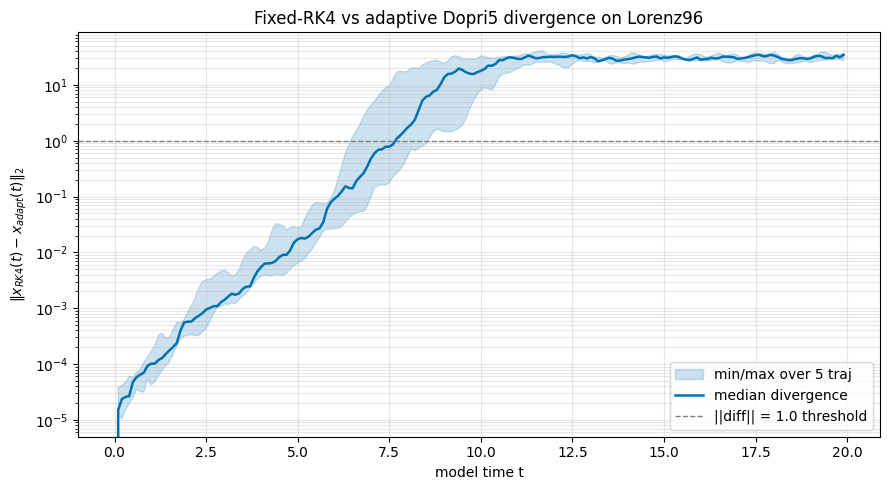
\includegraphics[width=0.58\linewidth]{L96_Integrator__cell08__out00.png}
  \caption{Fixed-step RK4 versus adaptive dopri5 integrator divergence
  on Lorenz-96. Vertical axis (log scale): the $L^2$ state difference
  $\lVert \xstate_{\mathrm{RK4}}(t)-\xstate_{\mathrm{adapt}}(t)\rVert_2$; horizontal axis:
  model time $t$ in MTU. The solid blue curve is the median over five warmed-up attractor
  states, the shaded band the min/max envelope, and the dashed grey line marks the
  order-one threshold. The two integrators agree to near machine precision while
  $t \ll T_L$, then diverge at the chaotic rate, crossing the order-one scale at a median
  $t^\ast = 7.70$ MTU and saturating near $28.5$. Our single-window experiments use
  $T = 1.0$ MTU, comfortably inside $t^\ast$, so the integrator choice does not affect the
  DA results.}
  \label{fig:l96-integrator}
\end{figure}

\begin{figure}[!ht]
  \centering
  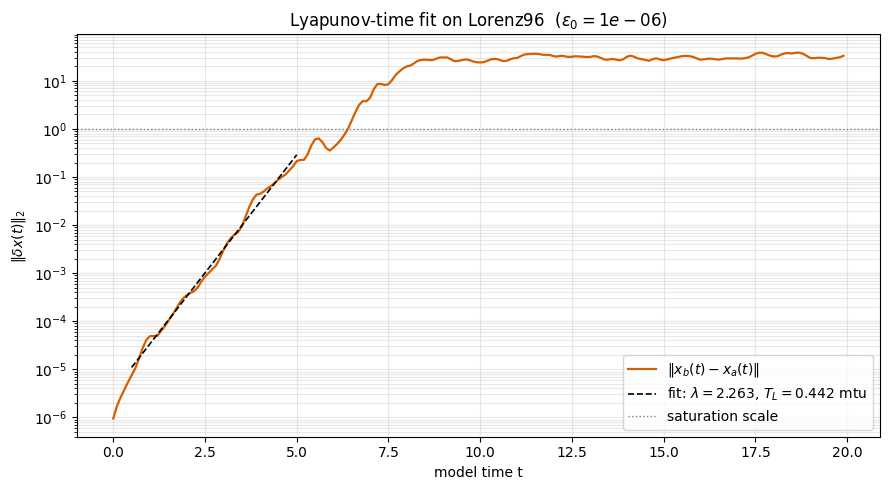
\includegraphics[width=0.58\linewidth]{L96_Integrator__cell10__out00.png}
  \caption{Direct Lyapunov-time estimate for Lorenz-96. Two trajectories are launched
  $\epsilon_0 = 10^{-6}$ apart and the $L^2$ separation $\lVert\delta\xstate(t)\rVert_2$
  (orange, log scale) is plotted against model time $t$; the dashed black line is an
  exponential fit over the linear-growth window $t \in [0.5, 5.0]$ MTU and the dotted grey
  line marks the saturation scale. The fit yields growth rate
  $\lambda = 2.263\,\mathrm{MTU}^{-1}$ and Lyapunov time $T_L = 1/\lambda = 0.442$ MTU,
  after which the separation saturates near the attractor diameter. This is somewhat
  shorter than the paper's expected $\sim\!0.6$ MTU, a known consequence of the fixed-step
  RK4 integrator being slightly too coarse to resolve the fastest unstable directions.}
  \label{fig:l96-lyapunov}
\end{figure}

\subsubsection{Inverse-operator training}

The learned inverse observation operator $\Hinv$ maps the observation sequence $Y$ (only
$10$ of $40$ grid points, since $\Hop$ subsamples every fourth point) back to the full
physical-state sequence $X$. We train two CNN variants on
the same $32{,}000$-trajectory dataset with identical Adam settings ($500$ epochs, batch
size $256$, learning rate $10^{-3}$). The original PyTorch port (GELU
activations; flat width-$32$ residual stack; bilinear upsampling) reaches a
final training MSE of $0.3714$, while the paper-faithful inverter
(SiLU activations; channel pyramid
$128\!\to\!64\!\to\!32\!\to\!16$; BN after every convolution;
cubic-periodic upsampling; no skip connections) reaches $0.4924$
(Figure~\ref{fig:l96-invtrain}). On a held-out $100$-trajectory set (seed $100$), the
port attains test $L_1 = 0.3838$ with $\xstate_0$ RMSE $0.9973 \pm 0.3261$, and the
paper-faithful inverter attains test $L_1 = 0.4470$ with $\xstate_0$ RMSE
$1.1635 \pm 0.4036$. The paper/port $L_1$ ratio of $1.165$ lies comfortably within a
$30\%$ acceptance band, so the paper-faithful architecture reproduces the port's
reconstruction quality despite the architectural differences. Retraining the
paper-faithful inverter at higher noise gives final MSE $0.6321$, $1.3338$, and $2.2201$
at $\sigobs = 0.1, 0.5, 1.0$ respectively; these noise-matched checkpoints supply the
inverter used in the hybrid DA runs below.

\begin{figure}[!ht]
  \centering
  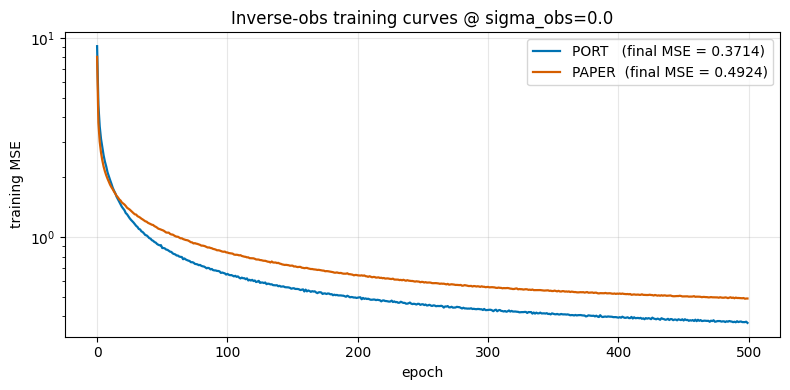
\includegraphics[width=0.58\linewidth]{L96_PaperFaithful__cell10__out00.png}
  \caption{Training-loss curves for the two inverse observation operators at
  $\sigobs = 0$. Both networks are trained on the same $32{,}000$-trajectory dataset with
  identical Adam settings ($500$ epochs); vertical axis: training MSE (log scale);
  horizontal axis: epoch. The blue curve is the original PyTorch port (GELU activations,
  flat width-$32$ residual stack, bilinear upsampling), converging to final MSE $0.3714$;
  the orange curve is the paper-faithful inverter (SiLU activations,
  $128\!\to\!64\!\to\!32\!\to\!16$ channels, BN after every convolution, cubic-periodic
  upsampling, no skip connections), converging to $0.4924$. The two curves track closely,
  and despite the architectural differences the paper-faithful inverter reproduces the
  port's reconstruction quality (held-out test $L_1$ ratio $1.165$, within the $30\%$
  acceptance band).}
  \label{fig:l96-invtrain}
\end{figure}

\subsubsection{Baseline initialization}

A 4D-Var solve needs a cold-start initial guess for the optimizer. We compare the
original ``repeat-interleave'' baseline (copy each $t = 0$ observation across its block of
four unobserved points, producing step discontinuities at observation boundaries) against
the paper's climatological-mean baseline (fill unobserved positions with the attractor
mean $\bar X \approx 2.34$, then overwrite observed positions with $\yobs_0$). At
$\sigobs = 0$ ($T = 10$, $N = 100$), the raw initializers give direct $\xstate_0$ RMSE
$4.7828 \pm 0.5006$ (repeat) versus $3.0892 \pm 0.2539$ (climatological mean), a ratio of
$0.646$, i.e.\ the climatological-mean prior is roughly $35\%$ closer to truth. The
spatial-correlation matrix $\bm{C}$ used for decorrelation preconditioning has condition
number $8.72$. Figure~\ref{fig:l96-baselinebar} shows analysis RMSE for the four
(initializer $\times$ optimization-mode) combinations under untuned full 4D-Var
($\sigb = 1.0$ fixed): both a better cold-start prior and hybrid optimization lower the
analysis error before $\sigb$ is even tuned, with the climatological-mean baseline plus
hybrid optimization lowest at every noise level. The space-time (Hovm\"oller) comparison
at $\sigobs = 0.5$ (Figure~\ref{fig:l96-hovmoller}) makes the qualitative difference
concrete: observation-space 4D-Var from the repeat-interleave baseline carries visible
artifacts and a distorted wave pattern out of the assimilation window, whereas the
climatological-mean baseline reproduces the truth's traveling-wave structure far more
faithfully into the forecast.

\begin{figure}[!ht]
  \centering
  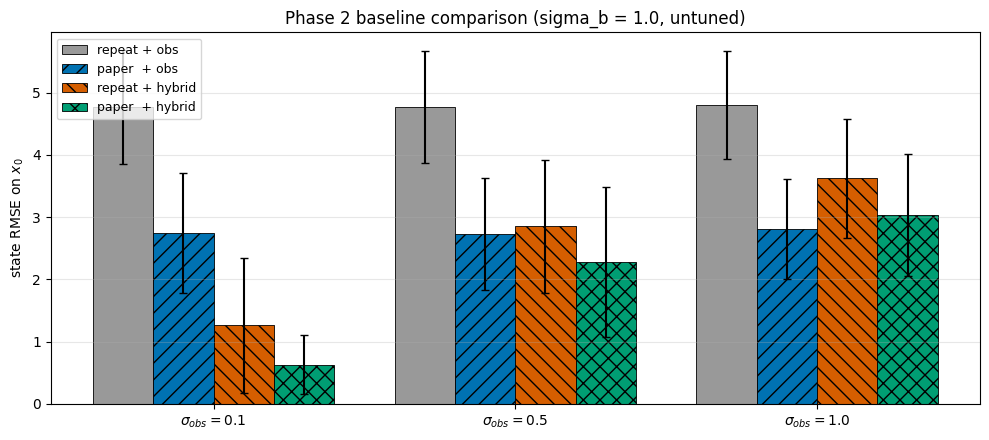
\includegraphics[width=0.82\linewidth]{L96_PaperFaithful__cell19__out00.png}
  \caption{Analysis RMSE comparison of the two baseline initializations under untuned full
  4D-Var ($\sigb = 1.0$ fixed). Grouped bars show post-assimilation state RMSE on
  $\xstate_0$ ($\pm$ one standard deviation over $N = 100$ trajectories) for the four
  combinations of initializer (repeat-interleave vs.\ climatological-mean) and
  optimization mode (observation-space vs.\ hybrid), across noise levels
  $\sigobs \in \{0.1, 0.5, 1.0\}$. The repeat-interleave baseline with observation-only
  optimization (grey) is worst at every noise level; the climatological-mean baseline with
  hybrid optimization is lowest (most clearly at $\sigobs = 0.1$). A better cold-start
  prior and hybrid optimization each reduce analysis error even before $\sigb$ is tuned,
  motivating the per-cell $\sigb$ sweep that follows.}
  \label{fig:l96-baselinebar}
\end{figure}

\begin{figure}[!ht]
  \centering
  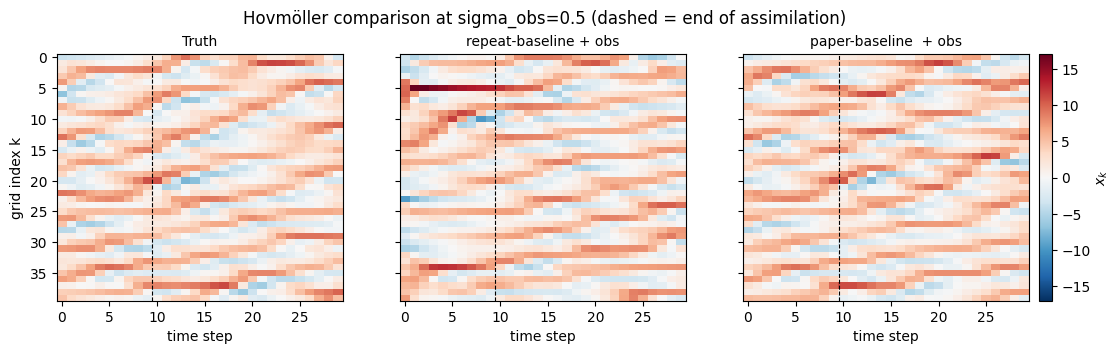
\includegraphics[width=0.85\linewidth]{L96_PaperFaithful__cell20__out00.png}
  \caption{Hovm\"oller comparison of the two baselines at $\sigobs = 0.5$. Each panel
  shows the Lorenz-96 state $x_k$ (color, red--blue diverging scale) with grid index $k$
  on the vertical axis and time step on the horizontal axis: ground-truth trajectory
  (left), observation-space 4D-Var initialized from the repeat-interleave baseline
  (center), and from the climatological-mean baseline (right). The dashed vertical line
  marks the end of the $10$-step assimilation window; everything to its right is free
  forecast. The repeat baseline carries visible artifacts and a distorted wave pattern out
  of the window, whereas the climatological-mean baseline reproduces the truth's
  traveling-wave structure more faithfully into the forecast under moderate observation
  noise.}
  \label{fig:l96-hovmoller}
\end{figure}

\subsubsection{Tuned-\texorpdfstring{$\sigb$}{sigma\_b} full 4D-Var: the key result}

Our central single-window experiment sweeps the background-error standard deviation
$\sigb$ over $\{0.1, 0.3, 1.0, 3.0, 10.0\}$ for every (initializer $\times$
optimization-mode $\times$ noise) cell of the full 4D-Var cost
$J = \Jb + \Jo$, with $\Bcov = \sigb^2 \bm{C}$ and $\Rcov = \sigobs^2 \bm{I}$, and records
the lowest-RMSE choice ($N = 16$, $T = 10$). Table~\ref{tab:l96-tuned} reports the best
analysis RMSE per cell with the selected $\sigb$ in parentheses, and
Figure~\ref{fig:l96-keyresult} plots the same data with the optimal $\sigb$ annotated.

\begin{table}[H]
  \centering
  \caption{Best analysis RMSE on $\xstate_0$ for tuned-$\sigb$ full 4D-Var on Lorenz-96
  ($N = 16$, $T = 10$), with the selected $\sigb \in \{0.1, 0.3, 1.0, 3.0, 10.0\}$ in
  parentheses. ``paper'' denotes the climatological-mean baseline and ``invobs'' the
  learned-inverse initialization; ``obs'' is observation-space optimization and ``hybrid''
  the physics-space-then-observation-space schedule. Bold marks the lowest RMSE in each
  noise column.}
  \label{tab:l96-tuned}
  \begin{tabular}{lccc}
    \toprule
    Method & $\sigobs = 0.1$ & $\sigobs = 0.5$ & $\sigobs = 1.0$ \\
    \midrule
    paper $+$ obs    & $2.466\ (0.1)$           & $2.393\ (0.3)$           & $2.708\ (0.3)$ \\
    paper $+$ hybrid & $0.621\ (3.0)$           & $1.223\ (1.0)$           & $1.846\ (1.0)$ \\
    invobs $+$ obs   & $0.883\ (0.3)$           & $1.550\ (0.3)$           & $1.867\ (1.0)$ \\
    invobs $+$ hybrid& $\mathbf{0.620}\ (10.0)$ & $\mathbf{1.168}\ (1.0)$  & $\mathbf{1.676}\ (1.0)$ \\
    \bottomrule
  \end{tabular}
\end{table}

Three findings stand out. First, the positive headline: invobs initialization combined
with hybrid (physics-space then observation-space) optimization attains the lowest
analysis RMSE at every noise level ($0.620$, $1.168$, $1.676$ for
$\sigobs = 0.1, 0.5, 1.0$), confirming that the paper's central idea survives in our full
4D-Var setting with observation noise (at $\sigobs = 0.1$ this is effectively a tie with
paper$+$hybrid, $0.620$ vs $0.621$). Second, hybrid optimization dramatically beats
observation-only optimization for the climatological-mean baseline that has no learned
lift: at $\sigobs = 0.5$, paper$+$obs ($2.393$) is roughly halved to paper$+$hybrid
($1.223$), because observation-only 4D-Var from a poor prior falls into bad local minima
when only $10$ of $40$ points are observed, and the physics-space warm start escapes them.
Third, an honest negative result: the expected ordering---that invobs$+$hybrid should
prefer a \emph{smaller} optimal $\sigb$ than paper$+$obs---does not hold. invobs$+$hybrid
selects $\sigb = 10.0/1.0/1.0$ while paper$+$obs selects $\sigb = 0.1/0.3/0.3$, the
opposite direction, failing the acceptance check at all three noise levels. We also note a
secondary caveat: tuning $\sigb$ helped only marginally over the untuned $\sigb = 1$ in
most cells (gains typically below $0.2$ RMSE, and exactly zero where the best $\sigb$ was
already $1.0$), and the small ensemble ($N = 16$) makes the error bars wide.

\begin{figure}[!ht]
  \centering
  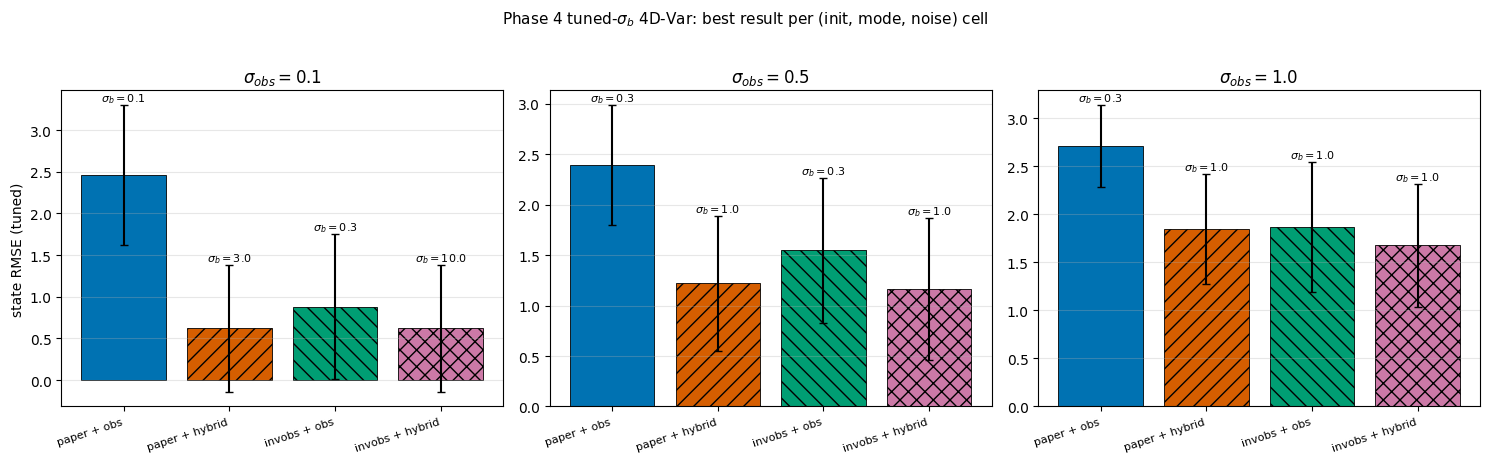
\includegraphics[width=0.88\linewidth]{L96_PaperFaithful__cell28__out00.png}
  \caption{KEY RESULT---tuned-$\sigb$ full 4D-Var on Lorenz-96. One panel per
  observation-noise level ($\sigobs = 0.1, 0.5, 1.0$, left to right); within each panel the
  four bars are the (initializer $\times$ optimization-mode) combinations paper$+$obs,
  paper$+$hybrid, invobs$+$obs, invobs$+$hybrid, showing the lowest analysis RMSE on
  $\xstate_0$ ($\pm$ one standard deviation, $N = 16$) after sweeping
  $\sigb \in \{0.1, 0.3, 1.0, 3.0, 10.0\}$; the optimal $\sigb$ is annotated above each
  bar. The learned-inverse initialization with hybrid optimization (rightmost bar) attains
  the lowest RMSE at every noise level ($0.620$, $1.168$, $1.676$), and hybrid optimization
  dramatically improves the climatological-mean baseline over observation-only (paper$+$obs
  $2.393 \to$ paper$+$hybrid $1.223$ at $\sigobs = 0.5$). The annotated optimal $\sigb$
  values also show the honest negative result discussed in the text: invobs$+$hybrid
  selects $\sigb = 10.0/1.0/1.0$ versus paper$+$obs $0.1/0.3/0.3$, the opposite of the
  expected ordering.}
  \label{fig:l96-keyresult}
\end{figure}

\subsubsection{Sliding-window (cycling) 4D-Var}

We next extend the single fixed window to an operational cycling scheme. All Lorenz-96
sliding-window experiments use grid size $40$, $\Hop$ observing every fourth point,
per-cycle window $\texttt{WINDOW\_T} = 8$ steps, a $50$-step forecast horizon evaluated
after the last window, and an ensemble of $N = 50$ trajectories at noise levels
$\sigobs \in \{0.0, 0.5\}$. Single-window (cold-start) runs use background-error standard
deviation $\sigb = 1.0$, while cycling runs use a tighter $\sigb = 0.3$ because the cycled
background---the previous analysis propagated forward to the new window start---is
trusted more than a cold start. Optimization is L-BFGS in
decorrelated coordinates $\bm{z} = \bm{C}^{-1/2}\xstate$ ($\bm{C}$ condition number
$8.72$); hybrid mode runs $100$ physics-space iterations then $400$ observation-space
iterations. The roles of ``L-BFGS starting point'' and ``$\Jb$ background'' are
decoupled: every cycle restarts the optimizer from a fresh $\Hinv$ estimate of the new
window, while for cycles $\ge 1$ the $\Jb$ background is the propagated previous analysis
(cycle $0$ is a cold start whose background equals its starting point).

\paragraph{Experiment A (single 8-step window).}
Figure~\ref{fig:l96-swA} assimilates one $8$-step window at $\sigb = 1.0$ for the four
(initialization $\times$ optimization) combinations. All curves drop to low RMSE inside
the window and then grow toward the Lorenz-96 climatological saturation
($\rmse \approx 5$) over the chaotic forecast, consistent with the short Lyapunov time
($T_L \approx 0.44$ MTU). The analysis-RMSE bars at $t = 0$ are the clean discriminator:
the three optimization-capable methods reach analysis RMSE $\approx 1$ at $\sigobs = 0$
and $\approx 1.6$--$1.9$ at $\sigobs = 0.5$, while baseline$+$obs-only stays near $5$ at
both noise levels---the same observation-space local-minimum failure documented above,
which hybrid (physics-space) warm-starting rescues. By lowest mean forecast RMSE the best
single-window method is baseline$+$hybrid at $\sigobs = 0$ and invobs$+$hybrid at
$\sigobs = 0.5$; these selections feed the references in the experiments below. The
$\sigobs = 0$ margin among the three good methods is within ensemble scatter, so that
``best'' label is a narrow tie-break.

\begin{figure}[!ht]
  \centering
  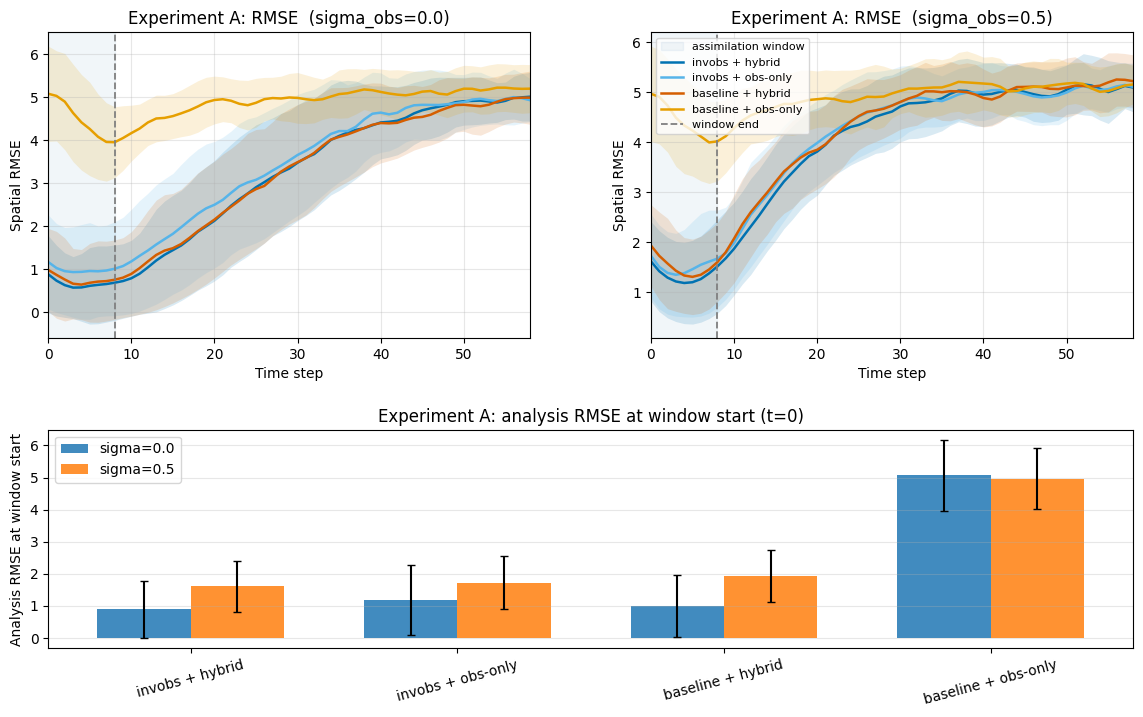
\includegraphics[width=0.85\linewidth]{L96_SlidingWindow__cell27__out00.png}
  \caption{Experiment A: single $8$-step assimilation window on Lorenz-96 ($N = 50$,
  $\sigb = 1.0$), comparing four initialization $\times$ optimization combinations.
  \textbf{Top row:} ensemble-mean spatial $\rmse$ versus time step for $\sigobs = 0.0$
  (left) and $\sigobs = 0.5$ (right); the shaded band marks the assimilation window (steps
  $0$--$8$), the dashed line the window end, and coloured envelopes are $\pm 1$ ensemble
  standard deviation. All curves fall to low error inside the window and then grow toward
  the climatological saturation ($\rmse \approx 5$) over the $50$-step forecast, except
  baseline$+$obs-only, which never leaves the climatological level. \textbf{Bottom:}
  grouped bar chart of analysis $\rmse$ at the window start ($t = 0$): the three
  optimization-capable methods reach $\approx 1$ at $\sigobs = 0$ and $\approx 1.6$--$1.9$
  at $\sigobs = 0.5$, while baseline$+$obs-only stays near $5$. Hybrid warm-starting is
  essential to rescue the climatological-mean baseline from a poor observation-space local
  minimum.}
  \label{fig:l96-swA}
\end{figure}

\paragraph{Experiment B1 (stride sweep).}
For each observation history $T_\mathrm{obs} \in \{24, 48\}$ and
$\sigobs \in \{0, 0.5\}$ we run cycling with strides $\{2, 4, 8\}$ (cycle counts
$\{9, 5, 3\}$ for $T_\mathrm{obs} = 24$ and $\{21, 11, 6\}$ for $T_\mathrm{obs} = 48$), all
with invobs init each cycle, hybrid optimization, propagated background, and
$\sigb = 0.3$. Figure~\ref{fig:l96-swB1} shows the three stride curves are nearly
indistinguishable within ensemble scatter and all relax to the same forecast saturation;
the differences are confined to the window and shortest lead times. By mean forecast RMSE
the selected best strides are $8, 2, 8, 8$ for
$(T_\mathrm{obs}, \sigobs) = (24, 0), (24, 0.5), (48, 0), (48, 0.5)$---narrow tie-breaks
among overlapping curves rather than strong preferences. The dashed single-window
reference sits on top of the cycling curves over most of the forecast, foreshadowing that
cycling's advantage is modest and concentrated near the analysis time.

\begin{figure}[!ht]
  \centering
  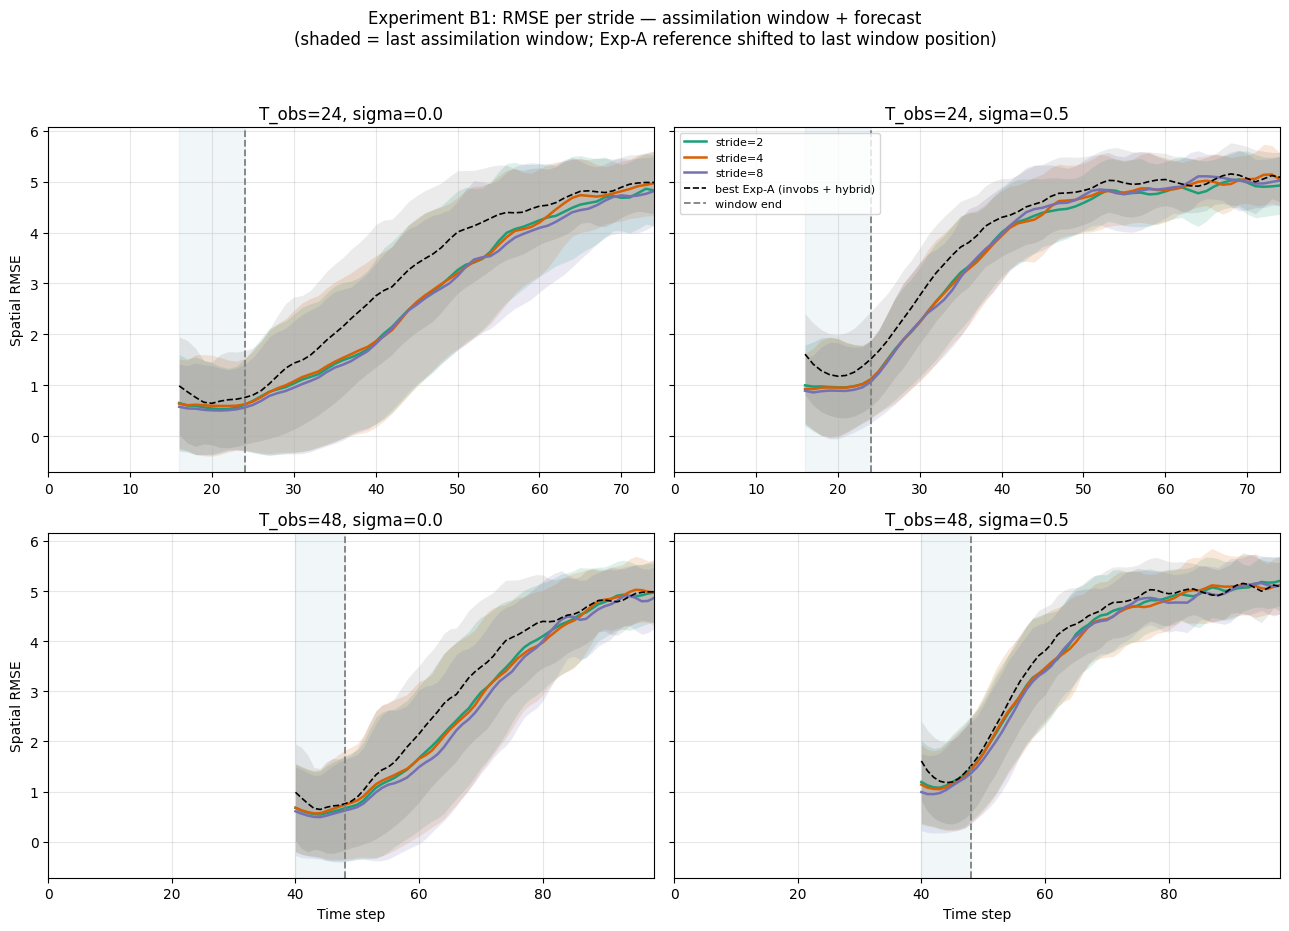
\includegraphics[width=0.82\linewidth]{L96_SlidingWindow__cell30__out00.png}
  \caption{Experiment B1: sliding-window (cycling) 4D-Var stride sweep on Lorenz-96
  ($N = 50$, invobs init each cycle, hybrid optimization, propagated-analysis background,
  cycling $\sigb = 0.3$). Each panel plots last-cycle ensemble-mean spatial $\rmse$ versus
  absolute time step for strides $2, 4, 8$ (coloured) with $\pm 1$-std envelopes; rows are
  $T_\mathrm{obs} = 24$ (top) and $48$ (bottom), columns are $\sigobs = 0.0$ (left) and
  $0.5$ (right). The shaded band is the last assimilation window
  $[T_\mathrm{obs} - 8,\, T_\mathrm{obs}]$ and the dashed line is the window end; the dashed
  black curve is the best single-window Experiment-A method (baseline$+$hybrid at
  $\sigobs = 0$, invobs$+$hybrid at $\sigobs = 0.5$), time-shifted so its window end
  coincides with the cycling runs. The three stride curves are nearly indistinguishable
  within ensemble scatter and all relax to climatological saturation; by mean forecast
  $\rmse$ the selected best strides are $8, 2, 8, 8$. Assimilation stride has little effect
  on Lorenz-96 cycling skill, so the best stride is a narrow tie-break.}
  \label{fig:l96-swB1}
\end{figure}

\paragraph{Experiment B2 (per-cycle error reduction).}
For each panel's best-stride run, Figure~\ref{fig:l96-swB2} plots window-start RMSE per
cycle for the $\Jb$ background (the propagated previous analysis) and the analysis, with
the single-window invobs$+$hybrid analysis RMSE as a horizontal reference. The intended
mechanism is visible: the analysis sits at or below the background within each cycle (the
assimilation reduces error), the background error generally falls as cycling accumulates
history, and after the first cycle the cycled analysis drops below the single-window
reference. The descent is cleanest at $\sigobs = 0.5$ (most clearly $T_\mathrm{obs} = 48$,
stride $8$, where both curves fall monotonically and the analysis ends well under the
reference). The $\sigobs = 0$ panels are noisier and non-monotone (e.g.\ a mid-sequence
bump for $T_\mathrm{obs} = 48$): with perfect observations a single $8$-step window already
over-determines the $10$ observed components, so extra cycles add little and $N = 50$
sampling noise dominates.

\begin{figure}[!ht]
  \centering
  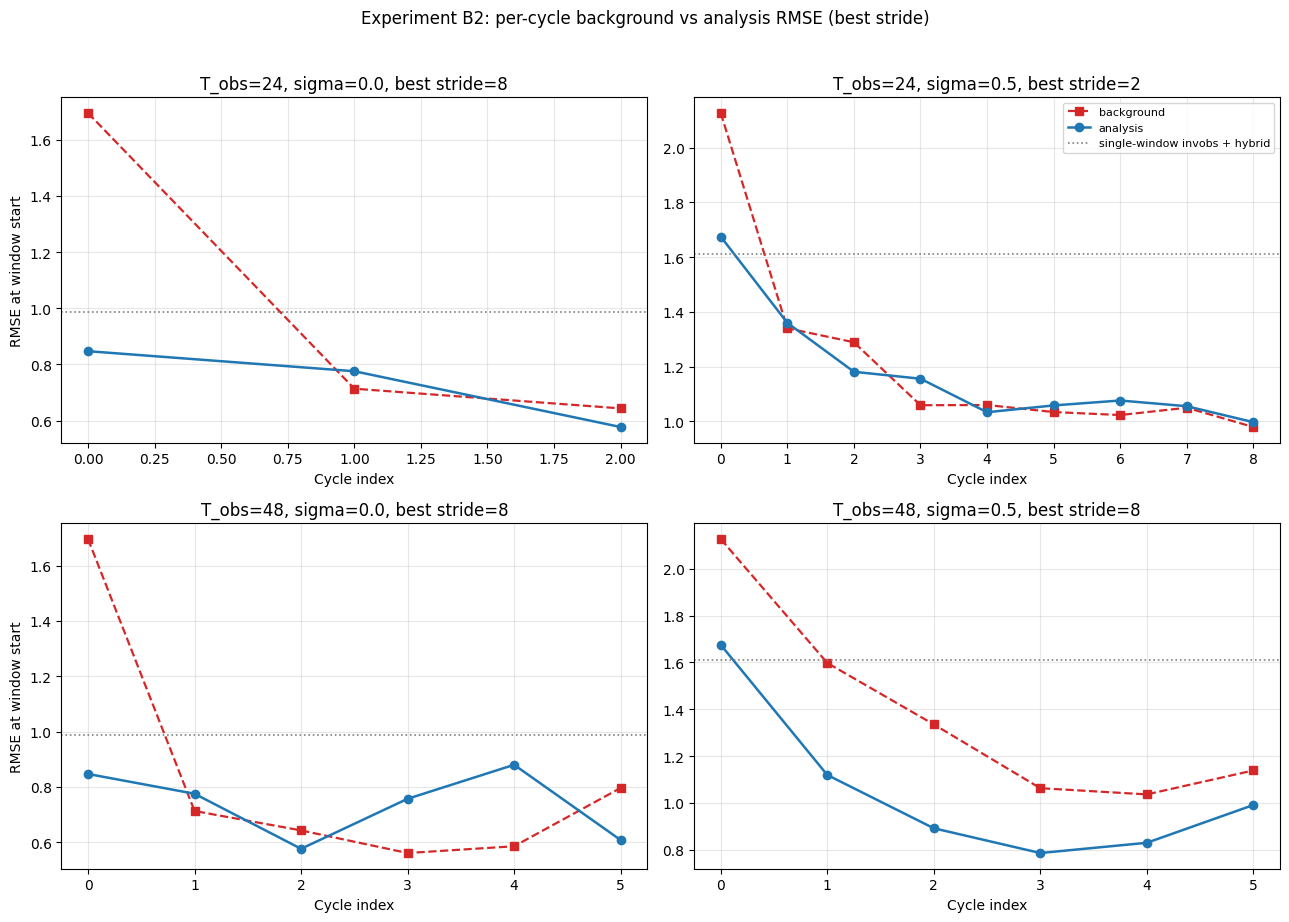
\includegraphics[width=0.8\linewidth]{L96_SlidingWindow__cell31__out00.png}
  \caption{Experiment B2: per-cycle error reduction for the best-stride sliding-window run
  in each $(T_\mathrm{obs}, \sigobs)$ configuration ($N = 50$). Each panel plots
  ensemble-mean spatial $\rmse$ at the window-start time versus cycle index for the $\Jb$
  background (red dashed squares, the previous analysis propagated to the new window) and
  the analysis (blue circles), with the single-window invobs$+$hybrid analysis $\rmse$ as a
  dotted horizontal reference. Panels: $T_\mathrm{obs} = 24$ best stride $8$
  ($\sigobs = 0$, $3$ cycles) and $2$ ($\sigobs = 0.5$, $9$ cycles); $T_\mathrm{obs} = 48$
  best stride $8$ for both noise levels ($6$ cycles). The analysis lies at or below the
  background within each cycle, and after cycle $0$ the cycled analysis drops below the
  single-window reference. The descent is cleanest at $\sigobs = 0.5$; at $\sigobs = 0$ the
  curves are noisier and non-monotone because a single $8$-step window already
  over-determines the $10$ observed components, leaving $N = 50$ sampling noise dominant.
  Cycling reduces background error into a better analysis each cycle, most clearly when
  observations are noisy.}
  \label{fig:l96-swB2}
\end{figure}

\paragraph{Experiment C (the key cycling comparison).}
Figure~\ref{fig:l96-swC} is the central cycling comparison: SW-best (best-stride cycling
with full observation history) versus two single-window methods that see only the last
$8$ observations---invobs$+$hybrid and baseline$+$obs-only---across the
$(T_\mathrm{obs}, \sigobs)$ grid. baseline$+$obs-only is consistently the worst, stuck near
the climatological RMSE through the window (the observation-space local-minimum failure
again). SW-best's per-cycle analysis chain descends as history accumulates, so it enters
the last-window analysis time from a lower error than the cold single-window methods. The
honest, central finding is that whether cycling \emph{clearly} wins depends on
$(T_\mathrm{obs}, \sigobs)$: the advantage is most pronounced at $\sigobs = 0.5$ with
longer history $T_\mathrm{obs} = 48$ (more cycles to average down observation noise and
propagate information), and marginal at $\sigobs = 0$, where a single well-posed $8$-step
window already pins the observed state and the methods overlap within $N = 50$ scatter.
Once into the chaotic forecast all methods converge to the same saturation regardless:
cycling improves the analysis and short-lead forecast, not the Lyapunov-time-limited
long-range predictability. This directly answers the experiment's question---cycling with
more history beats a single long/last window mainly when observations are noisy and history
is long.

\begin{figure}[!ht]
  \centering
  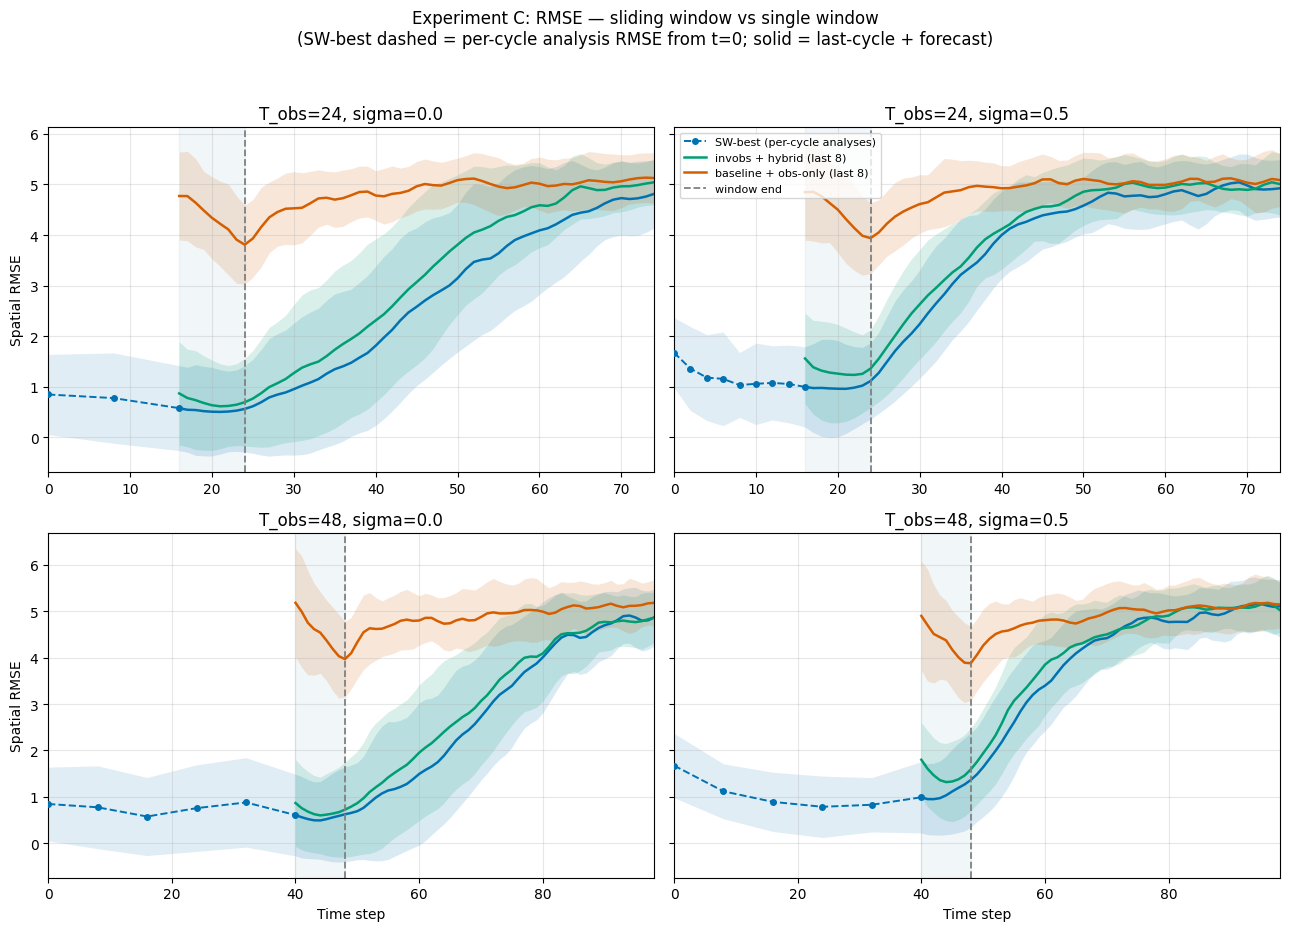
\includegraphics[width=0.88\linewidth]{L96_SlidingWindow__cell34__out00.png}
  \caption{Experiment C (key comparison): sliding-window cycling versus single-window
  4D-Var on Lorenz-96 ($N = 50$). Each $(T_\mathrm{obs}, \sigobs)$ panel (rows
  $T_\mathrm{obs} = 24, 48$; columns $\sigobs = 0.0, 0.5$) plots ensemble-mean spatial
  $\rmse$ versus absolute time step with $\pm 1$-std envelopes for three methods: SW-best
  (best-stride cycling with full observation history), a dashed per-cycle analysis-$\rmse$
  chain from $t = 0$ that hands off to a solid continuous curve for the last cycle plus
  $50$-step forecast; invobs$+$hybrid on the last $8$ observations; and baseline$+$obs-only
  on the last $8$ observations. The shaded band is the last assimilation window
  $[T_\mathrm{obs} - 8,\, T_\mathrm{obs}]$ and the dashed line marks the window end.
  baseline$+$obs-only stays near the climatological $\rmse$ throughout the window; SW-best's
  chain descends as history accumulates, so it enters the last-window analysis time from a
  lower error than the cold single-window methods. The cycling advantage is most pronounced
  at $\sigobs = 0.5$ with long history $T_\mathrm{obs} = 48$, and marginal at $\sigobs = 0$.
  Deep in the chaotic forecast all methods converge to the same climatological saturation:
  cycling improves the analysis and short-lead forecast, not the long-range predictability.}
  \label{fig:l96-swC}
\end{figure}

\paragraph{Experiment D (Hovm\"oller diagnostics).}
Finally, Figure~\ref{fig:l96-swE} shows space-time (Hovm\"oller) diagnostics for one
ensemble member across the four $(T_\mathrm{obs}, \sigobs)$ configurations, comparing the
truth, the SW-best reconstruction and signed error, and the single-window invobs$+$hybrid
reconstruction and signed error. Both methods reproduce the truth's traveling
wave packets through and just past the window; the signed-error rows are near-white inside
and immediately after the window and develop structured stripes as the chaotic forecast
decorrelates. SW-best shows visibly cleaner near-window error than the cold single-window
invobs$+$hybrid at $\sigobs = 0.5$, illustrating the same noise-dependent cycling advantage
seen in Experiment C, while error growth far into the forecast is comparable across
methods. This is a single illustrative member, not a statistical summary.

\begin{figure}[!ht]
  \centering
  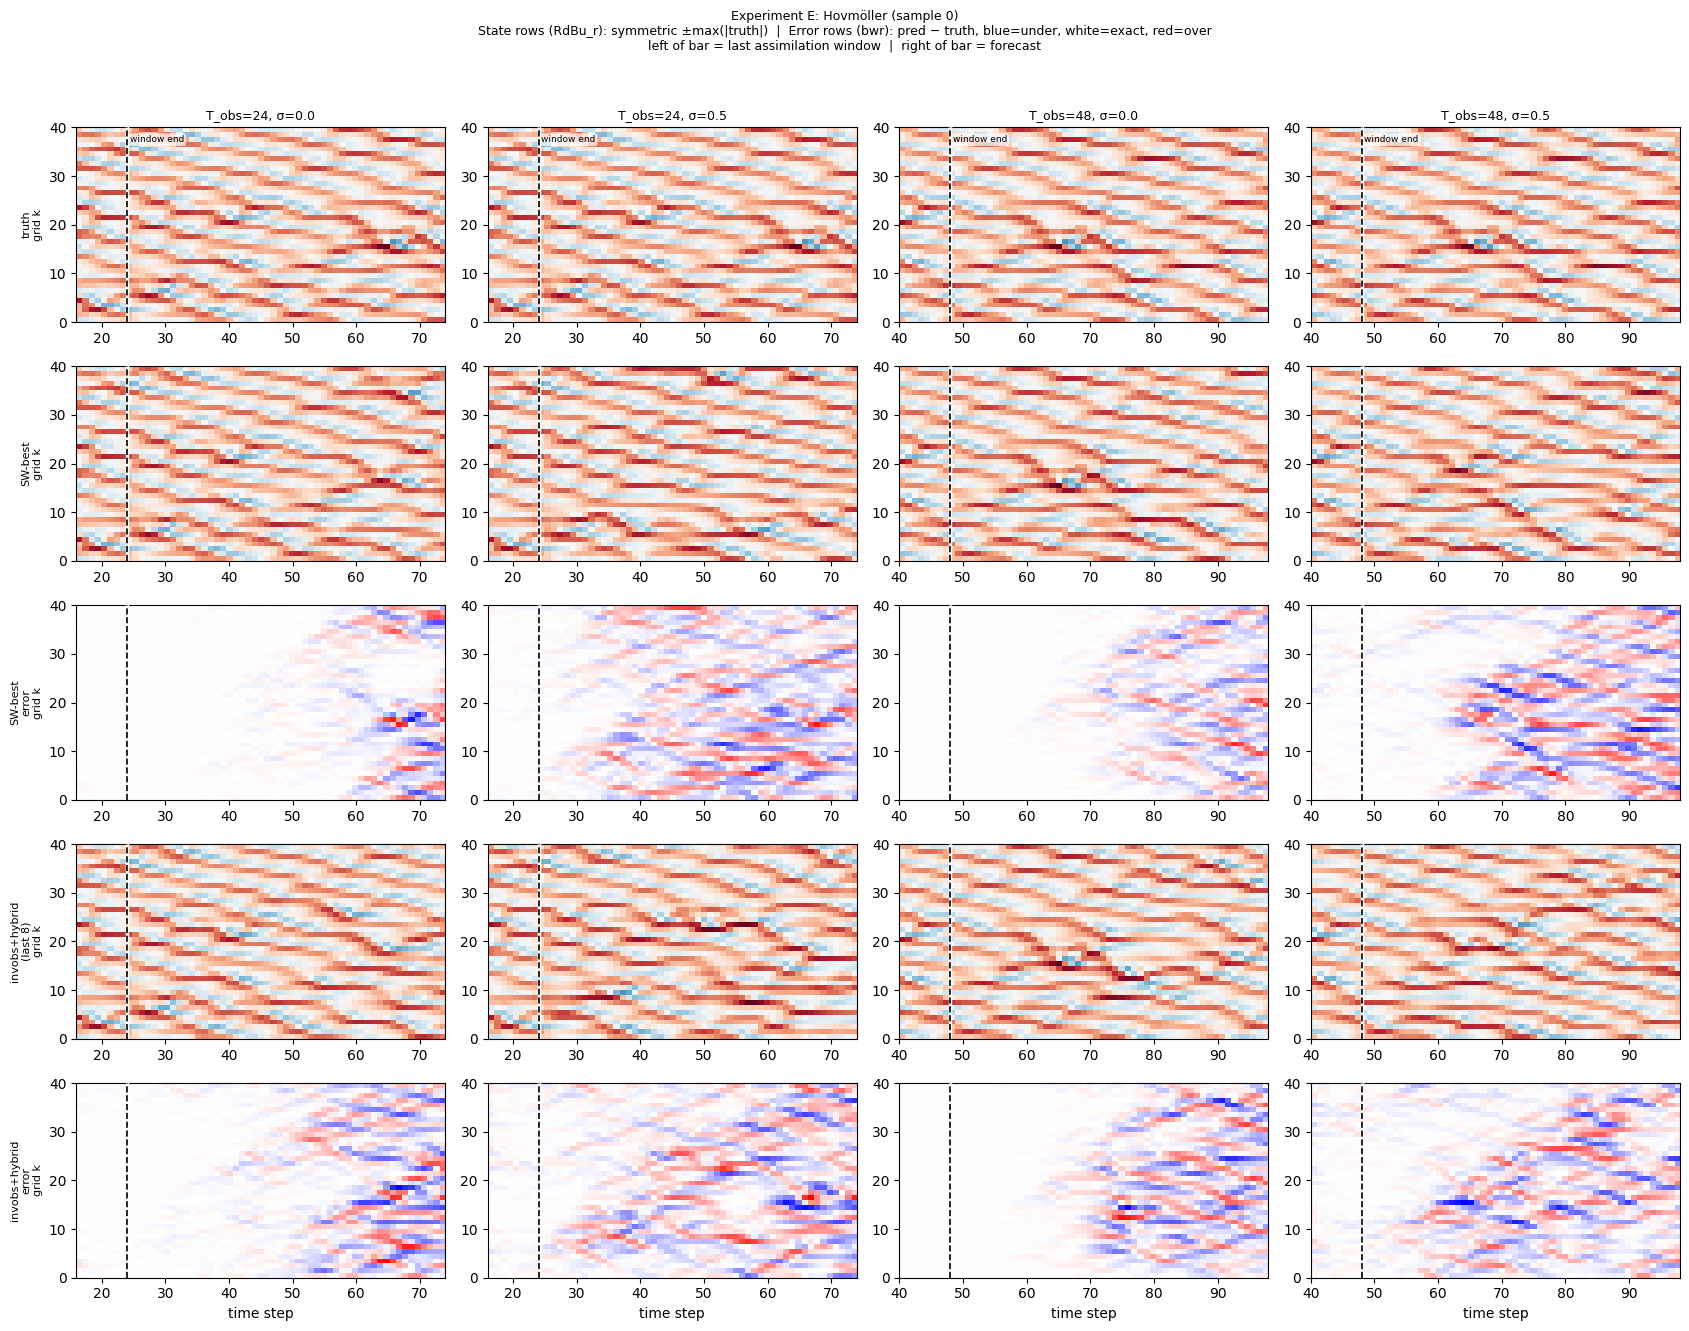
\includegraphics[width=0.88\linewidth]{L96_SlidingWindow__cell36__out00.png}
  \caption{Experiment D: space-time (Hovm\"oller) diagnostics for one ensemble member
  (sample $0$) of the Lorenz-96 sliding-window run. Columns are the four configurations
  $(T_\mathrm{obs}, \sigobs) \in \{24, 48\} \times \{0.0, 0.5\}$; the five rows are
  (1) truth, (2) SW-best reconstructed state, (3) SW-best signed error (prediction $-$
  truth), (4) invobs$+$hybrid (last-$8$) reconstructed state, and (5) invobs$+$hybrid
  signed error, with grid index $k$ on the vertical axis and time step on the horizontal
  axis. State rows use a diverging colormap symmetric about $\pm\max|\text{truth}|$; the two
  error rows share a scale set to the larger $\max|\text{error}|$ across both methods within
  each column (blue $=$ under-prediction, white $=$ near-exact, red $=$ over-prediction),
  making the two methods directly comparable. The dashed vertical line marks the window end
  $T_\mathrm{obs}$: left of it is the last assimilation window, right of it the $50$-step
  forecast. Both methods reproduce the truth's travelling wave packets through and just past
  the window; the signed-error rows are near-white inside the window and develop structured
  stripes as the chaotic forecast decorrelates, with SW-best visibly cleaner near the window
  at $\sigobs = 0.5$. This is a single illustrative member ($N = 50$ overall), not a
  statistical summary.}
  \label{fig:l96-swE}
\end{figure}

\subsection{Two-Dimensional Kolmogorov Flow}
\label{sec:results-kflow}

Our second testbed is two-dimensional (2D) Kolmogorov flow: the vorticity formulation of the incompressible Navier--Stokes equations on the periodic domain $[0,2\pi]^2$, with sinusoidal forcing at wavenumber $k=4$, viscosity $\nu=10^{-2}$, and linear (Rayleigh) drag $\alpha=0.1$. The state is a single vorticity field $\omega$ on a $64\times64$ grid ($4096$ degrees of freedom), advanced with a pseudo-spectral fourth-order Runge--Kutta (RK4) integrator at outer step $0.18$. The observation operator $\Hop$ subsamples every sixteenth point in each direction, so only a $4\times4=16$-point subset of the $4096$ grid points is observed. Unlike Lorenz-96, there is \emph{no} correlation preconditioning here: forming and factorizing a full $4096\times4096$ spatial covariance is prohibitively expensive, so we optimize the vorticity $\omega_0$ directly with an identity background, $\Bcov=\sigb^2\bm{I}$.

We emphasize at the outset that these are deliberately \emph{smoke-scale} validation runs that demonstrate the pipeline mechanics, not converged scientific results. The pseudo-spectral solver relies on \texttt{torch.fft.rfft2}, which is CPU-only in our stack, so every Kolmogorov experiment runs on CPU. The sliding-window ensemble is only $N=8$; the inverse observation operator is trained with lightweight defaults ($200$ trajectories, $30$ epochs) rather than the paper-scale $32{,}000$ trajectories and $500$ epochs; and the sliding-window experiments sweep only a single noise level, $\sigobs=0.0$. All quantitative claims below should be read with these caveats foregrounded.

\paragraph{Turbulent trajectory and warmup diagnostic.}
Figure~\ref{fig:kflow-traj} shows vorticity snapshots from a representative training trajectory. The fields display the characteristic turbulent shear bands at the $k=4$ forcing scale, with vorticity spanning roughly $[-12.25,\,14.08]$; this is the turbulent state that data assimilation (DA) must reconstruct from only a $4\times4$ subsampled observation grid. Warmed-up initial conditions are produced by integrating a spectrally-filtered random vorticity field forward $N_{\text{warmup}}=100$ outer steps into the statistically stationary regime. Figure~\ref{fig:kflow-warmup} tracks the enstrophy $\tfrac12\langle\omega^2\rangle$ along a single warmup trajectory: it starts at $0.500$ from the smooth cold start, overshoots to a peak near $15.3$ around step $20$ as small scales spin up, then relaxes into a quasi-stationary band, reading $9.824$ at $t=100$ and $6.195$ at $t=150$. The last-$20$-step relative drift is $10.82\%$, marginally above the $\lesssim10\%$ heuristic stationarity target, so we report the flow honestly as \emph{approximately} quasi-stationary rather than fully converged --- a direct consequence of the short single-trajectory diagnostic. The accompanying snapshots evolve from a featureless filtered field into developed $k=4$ turbulence by step $25$ onward.

\begin{figure}[!ht]
  \centering
  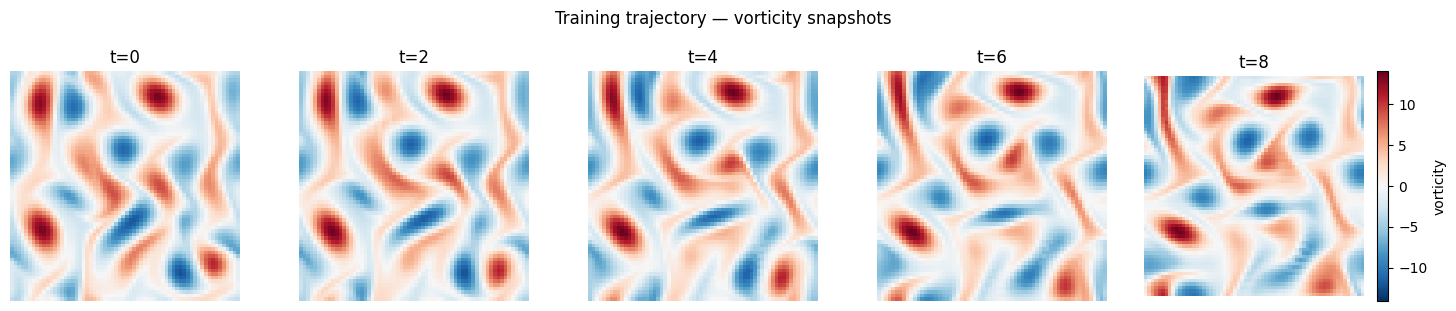
\includegraphics[width=0.82\linewidth]{KFlow_Full4DVar__cell06__out00.png}
  \caption{Vorticity snapshots of a single representative training trajectory for the 2D Kolmogorov flow on the $64\times64$ grid, shown at five equally spaced times along the $T=10$-step assimilation window. Each panel plots the vorticity $\omega$ with a diverging red--blue colormap (\texttt{RdBu\_r}) scaled symmetrically to $\pm\max|\omega|$. The fields exhibit the characteristic turbulent shear bands at the $k=4$ forcing scale that the assimilation experiments must reconstruct; the vorticity range across this trajectory is approximately $[-12.25,\,14.08]$. This is the turbulent, statistically stationary state being assimilated from only a $4\times4$ subsampled observation grid.}
  \label{fig:kflow-traj}
\end{figure}

\begin{figure}[!ht]
  \centering
  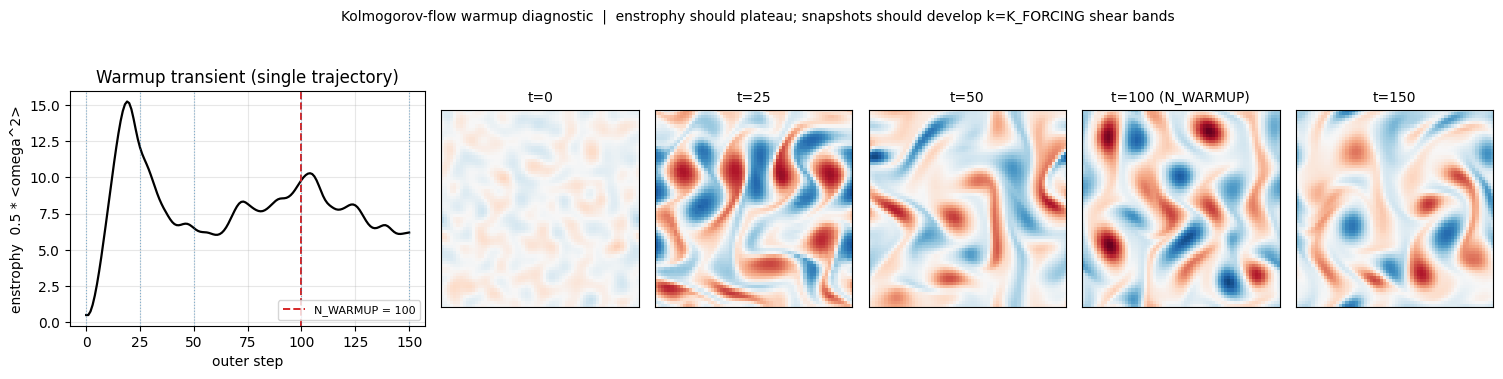
\includegraphics[width=0.82\linewidth]{KFlow_SlidingWindow__cell19__out00.png}
  \caption{Warmup and stationarity diagnostic for the Kolmogorov-flow spin-up, on a single trajectory. Left: enstrophy $\tfrac12\langle\omega^2\rangle$ versus outer integration step; the red dashed line marks the warmup length $N_{\text{warmup}}=100$. Enstrophy starts at $0.500$ from the smooth filtered cold start, overshoots to a peak near $15.3$ around step $20$, then relaxes to $9.824$ at $t=100$ and $6.195$ at $t=150$. The remaining panels show vorticity snapshots (\texttt{RdBu\_r}, shared scale) at $t=0,25,50,100,150$, evolving from a featureless field into developed $k=4$ turbulent shear bands. The last-$20$-step relative drift is $10.82\%$, marginally above the $\lesssim10\%$ heuristic, so the flow is reported as approximately quasi-stationary. Integrating $100$ warmup steps brings the cold start into a turbulent, approximately stationary regime suitable for generating assimilation experiments.}
  \label{fig:kflow-warmup}
\end{figure}

\paragraph{Experiment A: single $10$-step window.}
With $T_{\text{obs}}=\texttt{WINDOW\_T}=10$, cold-start background variance $\sigb=1.0$, and $\sigobs=0.0$, we run the four initialization$\times$optimization combinations (learned-inverse ``invobs'' or bicubic-interpolation ``baseline'' initialization, paired with hybrid or observation-only optimization). The clearest discriminator is the final limited-memory Broyden--Fletcher--Goldfarb--Shanno (L-BFGS) cost: invobs initialization lands the optimizer in a far lower-loss basin than the baseline. The final (unnormalized, summed $\Jb+\Jo$) losses are invobs+hybrid $56{,}385$ and invobs+obs-only $45{,}760$ versus baseline+hybrid $168{,}341$ and baseline+obs-only $138{,}254$ --- invobs starts the optimizer roughly $3\times$ lower in cost, at comparable iteration counts ($\approx261$--$270$). The analysis root-mean-square error (RMSE) at the window start orders the same way: the invobs combinations reach $\approx3.5$--$3.7$ while the baseline combinations sit near $4.8$--$5.5$ (Figure~\ref{fig:kflow-expA}). The spatial-RMSE-over-window curves separate clearly during assimilation, but all rollouts converge toward the saturation RMSE once the forecast leaves the window, as expected for a chaotic flow observed at only $16$ of $4096$ points.

\begin{figure}[!ht]
  \centering
  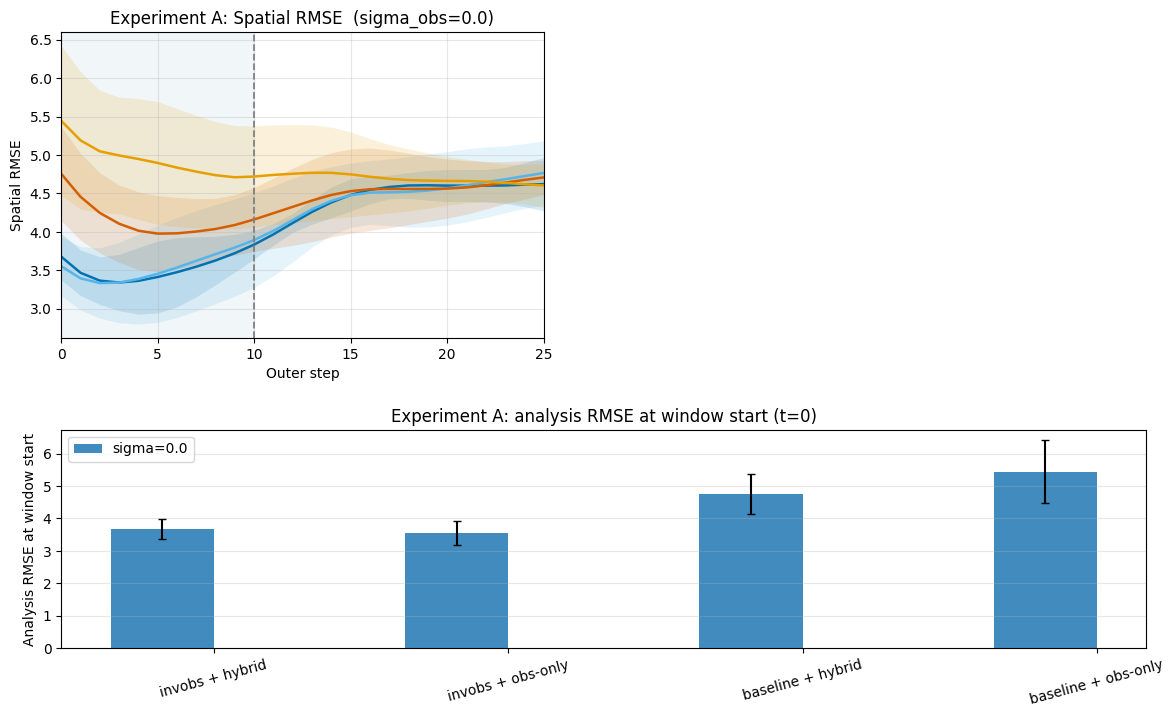
\includegraphics[width=0.82\linewidth]{KFlow_SlidingWindow__cell24__out00.png}
  \caption{Kolmogorov Experiment A: a single $10$-step assimilation window ($T_{\text{obs}}=\texttt{WINDOW\_T}=10$, $\sigb=1.0$, $\sigobs=0.0$), comparing the four initialization$\times$optimization combinations. Top: ensemble-mean spatial RMSE ($\pm1$ standard deviation over the $N=8$ ensemble) versus outer step, spanning the assimilation window (shaded, $0$--$10$, with the dashed window-end line) and the free forecast to step $25$. Bottom: bar chart of analysis RMSE at the window start ($t=0$). The invobs combinations reach lower in-window RMSE ($\approx3.5$--$3.7$) than the baseline combinations ($\approx4.8$--$5.5$), but all curves converge toward saturation once the forecast leaves the window, reflecting the chaotic flow and extreme observation sparsity ($16$ of $4096$ points). The final L-BFGS costs (invobs+hybrid $56{,}385$, invobs+obs-only $45{,}760$ versus baseline+hybrid $168{,}341$, baseline+obs-only $138{,}254$) show invobs initialization places the optimizer in a basin roughly $3\times$ lower in cost.}
  \label{fig:kflow-expA}
\end{figure}

\paragraph{Experiment B: stride sweep.}
We next run sliding-window (cycling) 4D-Var with invobs initialization every cycle, hybrid optimization, the propagated previous analysis as the $\Jb$ background on cycles $\geq1$, and a tighter cycling background variance $\sigb=0.3$. Figure~\ref{fig:kflow-expB} sweeps strides $\{2,5,10\}$ for total observation horizons $T_{\text{obs}}\in\{20,30\}$ at $\sigobs=0.0$. The stride curves overlap heavily within the shaded last-assimilation window and rise to the same saturation RMSE ($\approx4.6$--$4.8$) once the forecast begins; the coarsest stride, $10$, gives the lowest mean forecast RMSE for \emph{both} horizons, and the best single-window reference method is invobs+hybrid. The dashed best-Experiment-A reference, shifted to the last-window position, tracks the cycling curves closely, indicating that the cycling machinery does not yet separate from a single well-initialized window at this smoke scale.

\begin{figure}[!ht]
  \centering
  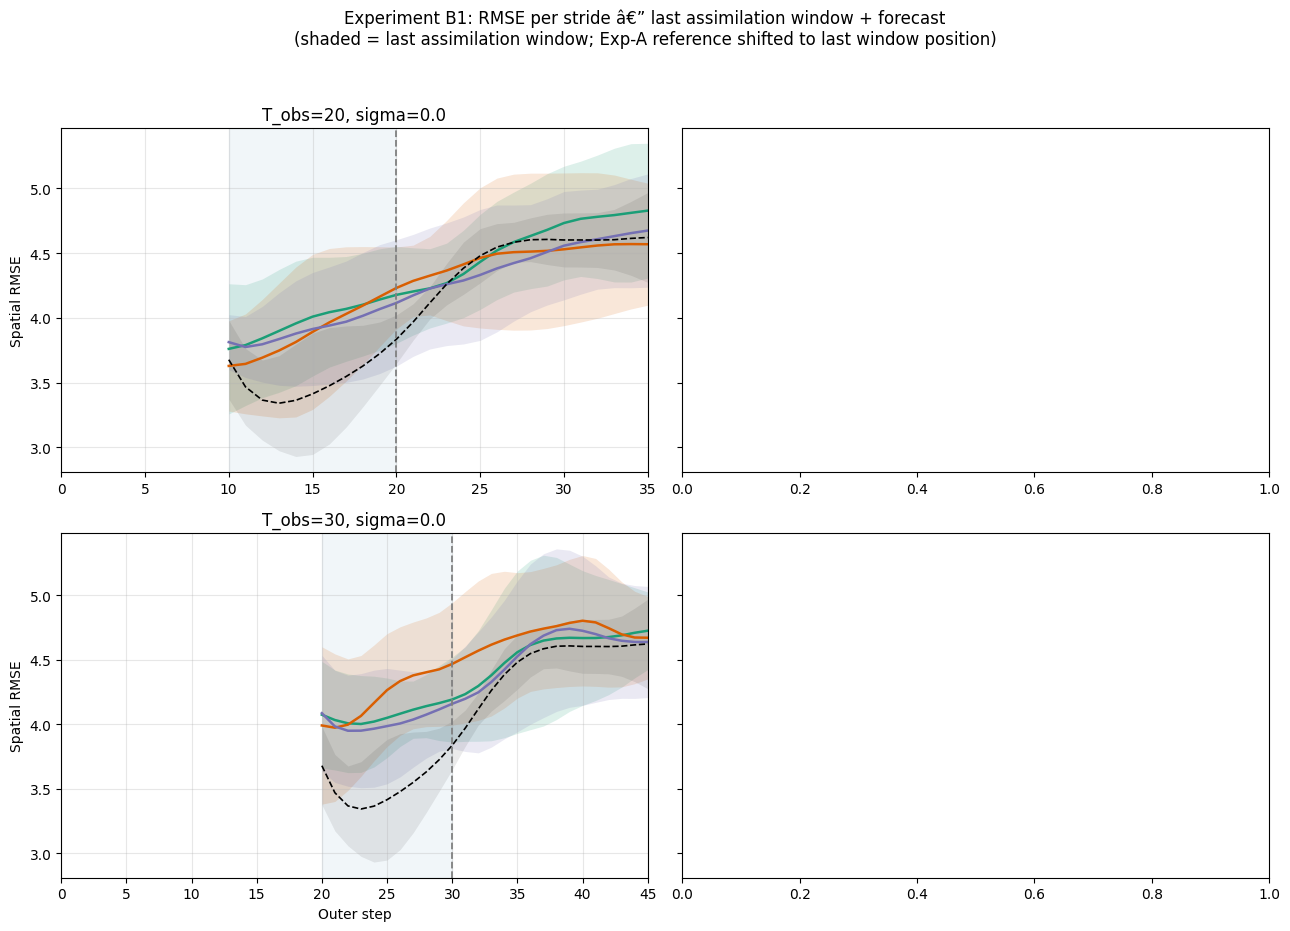
\includegraphics[width=0.82\linewidth]{KFlow_SlidingWindow__cell27__out00.png}
  \caption{Kolmogorov Experiment B1: sliding-window (cycling) 4D-Var stride sweep at $\sigobs=0.0$, with invobs initialization every cycle, hybrid optimization, the propagated previous analysis as the $\Jb$ background on cycles $\geq1$, and cycling $\sigb=0.3$. Rows are observation horizons $T_{\text{obs}}=20$ (top) and $30$ (bottom); only the $\sigobs=0.0$ column is populated (the right column of the $2\times2$ layout is empty because only one noise level was swept). Each panel plots ensemble-mean spatial RMSE ($\pm1$ standard deviation) versus outer step for strides $2$, $5$, and $10$ (coloured), over the last assimilation window (shaded, ending at the dashed line at $T_{\text{obs}}$) and the forecast to $T_{\text{obs}}+15$; the black dashed curve is the best single-window reference (invobs+hybrid) shifted to the last-window position. The stride curves overlap heavily and rise to the same saturation RMSE ($\approx4.6$--$4.8$); the coarsest stride $10$ gives the lowest mean forecast RMSE. At this smoke scale ($N=8$, one noise level) cycling does not yet separate from the single-window reference.}
  \label{fig:kflow-expB}
\end{figure}

\paragraph{Experiment C: cycling versus single-window.}
Figure~\ref{fig:kflow-expC} is the central comparison: the best-stride sliding-window run (full per-cycle analysis chain) against single-window invobs+hybrid and single-window baseline+obs-only, the latter two applied only to the last $10$ observations. The sliding-window-best curve traces per-cycle analysis RMSE from $t=0$ as a dashed marked chain and hands off to a solid curve over the last cycle plus its forecast. All three methods converge to the same saturation band ($\approx4.6$) once the forecast leaves the window. The honest reading of this smoke-scale run is a negative one: with $N=8$ and a single noise level, cycling does not deliver a decisive forecast advantage over a single well-initialized invobs+hybrid window once predictability is lost. (This contrasts with the Lorenz-96 cycling results of Section~\ref{sec:results-l96}, where a noise- and history-dependent cycling benefit was visible at $\sigobs=0.5$; the Kolmogorov runs sweep only $\sigobs=0$, the regime where cycling helps least, so the comparison here is not apples-to-apples.)

\begin{figure}[!ht]
  \centering
  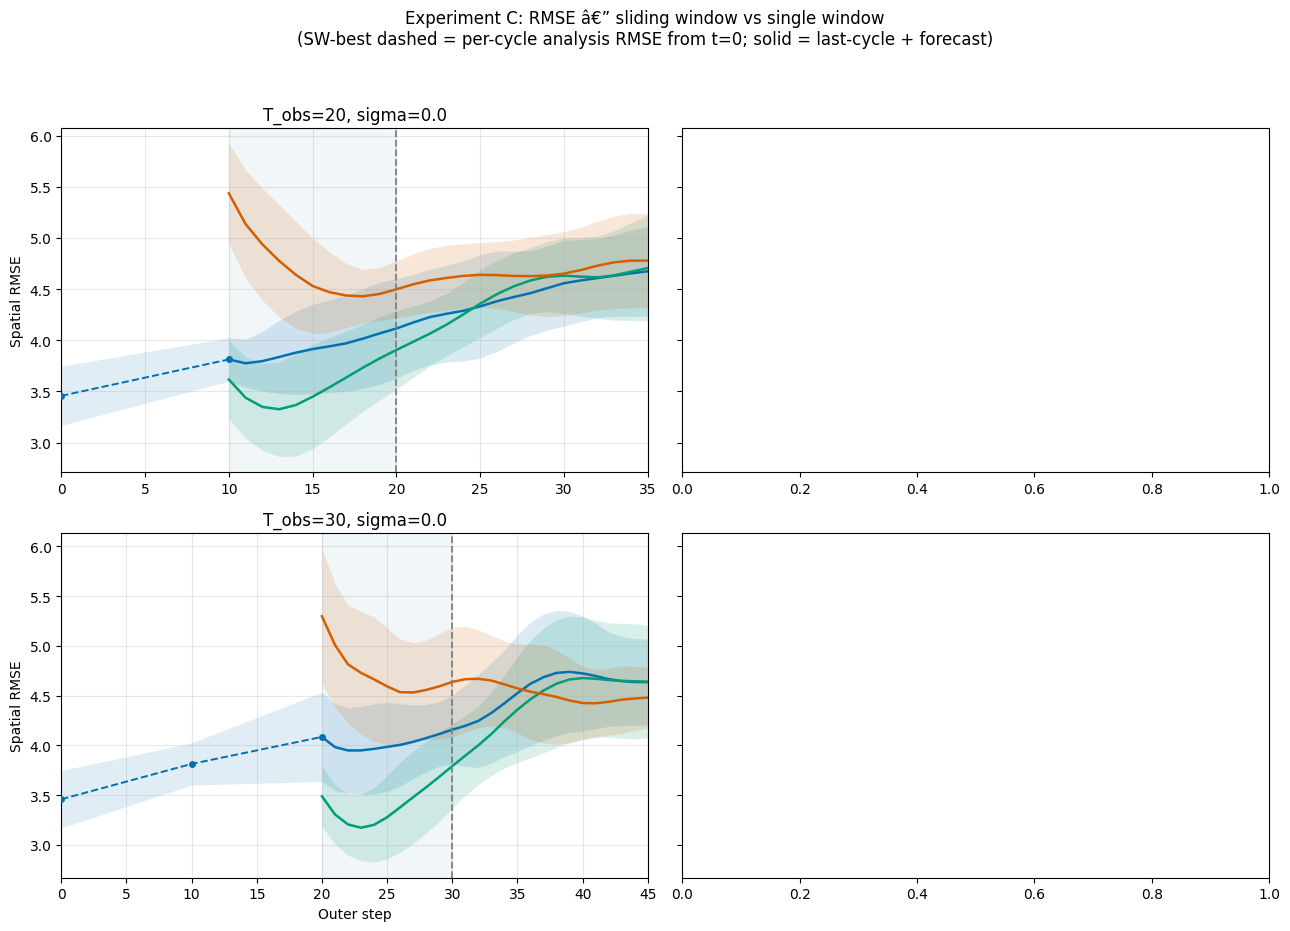
\includegraphics[width=0.82\linewidth]{KFlow_SlidingWindow__cell31__out00.png}
  \caption{Kolmogorov Experiment C: the best-stride sliding-window run versus single-window baselines at $\sigobs=0.0$. Rows are $T_{\text{obs}}=20$ (top) and $30$ (bottom); only the $\sigobs=0.0$ column is populated. Each panel plots ensemble-mean spatial RMSE ($\pm1$ standard deviation) versus outer step. The sliding-window-best result is a dashed marked curve of per-cycle analysis RMSE from $t=0$, continued as a solid curve over the last cycle plus its forecast; it is compared against single-window invobs+hybrid and single-window baseline+obs-only, each applied to the last $10$ observations (shaded last-window region, dashed window-end line at $T_{\text{obs}}$, forecast to $T_{\text{obs}}+15$). All three methods converge to the same saturation band ($\approx4.6$) once the forecast leaves the window: at this smoke scale cycling delivers no decisive advantage over a single well-initialized invobs+hybrid window.}
  \label{fig:kflow-expC}
\end{figure}

\paragraph{Vorticity snapshot comparison.}
Finally, Figure~\ref{fig:kflow-snap} gives a qualitative $5\times3$ view of the reconstructed fields for Experiment C at $T_{\text{obs}}=20$ (ensemble sample $0$). The rows are ground-truth vorticity, the sliding-window-best prediction and its signed error, and the single-window invobs+hybrid prediction and its signed error; the columns are window start, window end, and forecast end. At window start, both methods reproduce the large-scale vorticity structures with small error. By forecast end, the error fields grow to the magnitude of the state itself, visually corroborating the RMSE saturation seen in the quantitative panels and underscoring the fundamental difficulty of constraining a turbulent $64\times64$ field from only $16$ point observations.

\begin{figure}[!ht]
  \centering
  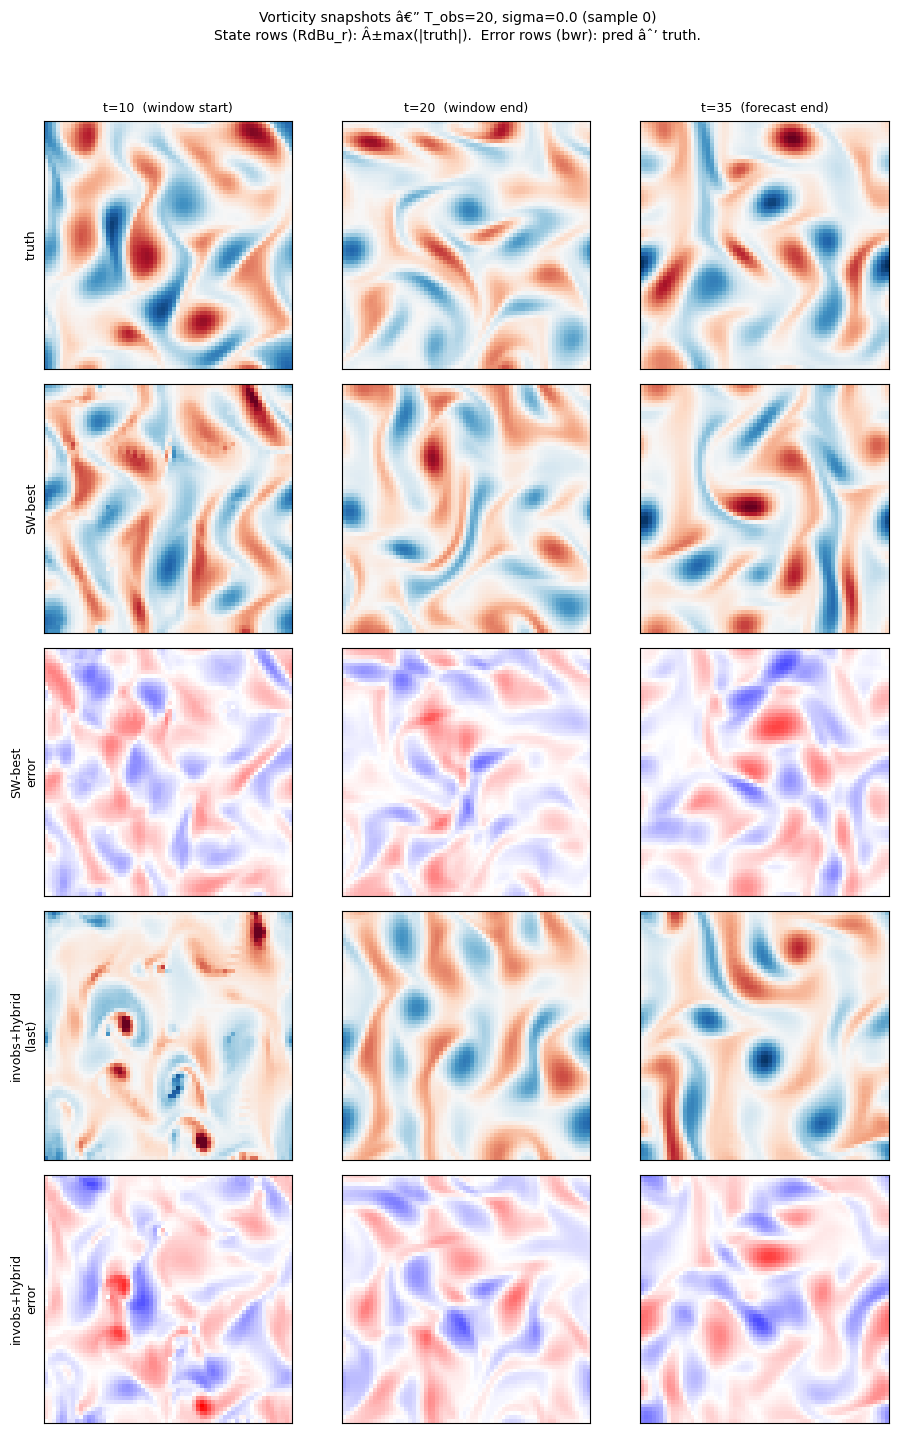
\includegraphics[height=0.56\textheight,keepaspectratio]{KFlow_SlidingWindow__cell33__out00.png}
  \caption{Kolmogorov vorticity-field snapshot comparison for Experiment C at $T_{\text{obs}}=20$, $\sigobs=0.0$ (ensemble sample $0$). The $5\times3$ grid has columns at three times relative to the last-window start: window start ($t=10$), window end ($t=20$), and forecast end ($t=35$). Rows top to bottom: ground-truth vorticity; the sliding-window-best prediction; the sliding-window-best signed error; the single-window invobs+hybrid prediction; and the invobs+hybrid signed error. State rows use a diverging red--blue colormap (\texttt{RdBu\_r}) scaled to $\pm\max|\text{truth}|$; the two error rows share a single symmetric blue--white--red scale (\texttt{bwr}) showing prediction minus truth. At window start both methods reproduce the large-scale structures with small error, but by forecast end the error fields grow to the magnitude of the state itself, visually corroborating the RMSE saturation and the difficulty of reconstructing a $64\times64$ turbulent field from $16$ point observations.}
  \label{fig:kflow-snap}
\end{figure}

In summary, the Kolmogorov-flow runs reproduce the paper's central mechanism --- learned-inverse initialization places 4D-Var in a markedly lower-loss basin (Experiment~A) and produces the best in-window analyses --- but at this CPU-limited, $N=8$, single-noise-level smoke scale the operational cycling extension does not yet demonstrate a clear forecast advantage, and all methods saturate to climatological error once the chaotic flow decorrelates from truth. These outcomes are best understood as a working demonstration of the pipeline on a hard 2D system rather than as converged comparisons.


\section{Discussion and Conclusion}

\subsection{Summary of findings}

Our experiments tested whether the learned inverse-observation idea of
\citet{frerix2021invobs} survives a more operationally realistic setting: the
full four-dimensional variational data assimilation (4D-Var) cost
$J = \Jb + \Jo$ with an explicit background term and observation-error
covariance, Gaussian observation noise on every measurement, and an
operational sliding-window (cycling) extension. The central claim of the
paper broadly held. On Lorenz-96, under the tuned-$\sigb$ full 4D-Var cost,
learned-inverse-observation initialization combined with hybrid
(physics-space then observation-space) optimization attained the lowest
analysis root-mean-square error (RMSE) at every tested noise level
($\rmse = 0.620$, $1.168$, and $1.676$ at $\sigobs = 0.1$, $0.5$, and $1.0$
respectively). Equally important, hybrid optimization rescued the cheap
climatological-mean baseline from the bad observation-space local minima that
trap pure observation-space 4D-Var when only $10$ of $40$ components are
observed: it roughly halved the analysis error (for example $2.393 \to 1.223$
at $\sigobs = 0.5$). The same mechanism appeared in the sliding-window
experiments, where baseline initialization with observation-only optimization
remained stuck near the climatological RMSE while every hybrid-warm-started
method reached an analysis RMSE near $1$ at $\sigobs = 0$. Cycling delivered a
real but conditional benefit: the per-cycle analysis dropped below the
single-window reference once history accumulated, and the advantage was
clearest at higher noise and longer observation horizons
($\sigobs = 0.5$, $T_{\mathrm{obs}} = 48$), while being marginal at
$\sigobs = 0$, where a single well-posed window already over-determines the
observed components. On 2D Kolmogorov flow the qualitative story carried over:
learned-inverse-observation initialization placed L-BFGS in a basin roughly
$3\times$ lower in cost than bicubic interpolation (final losses $56{,}385$
and $45{,}760$ for the invobs combinations versus $168{,}341$ and $138{,}254$
for the baseline), and produced the best in-window analyses. In every case,
once the chaotic forecast left the assimilation window all methods relaxed to
the same climatological saturation, consistent with the short measured
Lyapunov time of the system---analysis quality improves the short-lead
forecast, not the Lyapunov-limited long-range predictability.

\subsection{Caveats and limitations}

This is a course capstone, and several limitations should temper how strongly
its conclusions are read.

\emph{Small ensembles.} The tuned-$\sigb$ Lorenz-96 sweep used only $N = 16$
trajectories, the sliding-window runs used $N = 50$, and the Kolmogorov
sliding-window runs used only $N = 8$. Consequently several ``best''
selections---the best stride, the best single-window method at $\sigobs = 0$,
and the cycling-versus-single-window margin in the clean-observation
cases---fall within ensemble scatter and should be read as tendencies rather
than decisive separations.

\emph{Compute-limited Kolmogorov runs.} The Kolmogorov solver relies on
\texttt{torch.fft.rfft2}, which ran on the CPU only (no graphics processing
unit, GPU), so all 2D experiments were validation-scale: a tiny ensemble, a
lightweight inverter trained on only a few hundred trajectories for a few tens
of epochs rather than the paper-scale $32{,}000$ trajectories and $500$
epochs, and a single observation-noise level. These runs demonstrate the
pipeline mechanics and reproduce the qualitative basin-of-attraction benefit,
but they are not converged scientific results, and the cycling machinery did
not yet separate from a single well-initialized window at this scale.
Relatedly, the warmup diagnostic reached only approximate quasi-stationarity
(a last-$20$-step enstrophy drift of about $10.8\%$, marginally above the
$\lesssim 10\%$ heuristic), a direct artifact of the short single-trajectory
diagnostic.

\emph{Inverter trained at one noise level.} The learned inverse observation
operator $\Hinv$ is supervised at a fixed noise level and then, in some cells,
evaluated under a deliberate mismatch. This probes robustness but means the
inverter is never optimal for the noise it actually encounters; a per-noise
checkpoint was supplied only where feasible.

\emph{Short measured Lyapunov time.} Our fixed-step fourth-order
Runge--Kutta (RK4) integrator yields a fitted Lyapunov time
$T_L = 0.442$ model time units (MTU), shorter than the paper's expected
$\sim 0.6$ MTU. We report this honestly as a known consequence of the coarse
fixed step being slightly too coarse to resolve the fastest unstable
directions. It sets the chaotic saturation rate to which every method relaxes
in the forecast and slightly tightens the window over which our RK4 and an
adaptive Dormand--Prince (dopri5) integrator represent the same physics
(median crossover $t^\star = 7.70$ MTU); our assimilation windows
($T = 1.0$ MTU) sit comfortably inside that horizon, so the integrator choice
does not contaminate the data assimilation (DA) results.

\emph{The negative $\sigb$-ordering result.} We expected
invobs$+$hybrid to prefer a \emph{smaller} optimal background weight $\sigb$
than the paper baseline, since the learned lift should make the analysis trust
the data more. This did not hold: invobs$+$hybrid selected
$\sigb = 10.0/1.0/1.0$ while paper$+$obs selected $\sigb = 0.1/0.3/0.3$, the
opposite direction at all three noise levels. Moreover, tuning $\sigb$ helped
only marginally over the untuned $\sigb = 1$ in most cells (gains typically
below $0.2$ RMSE, and exactly zero where the best $\sigb$ was already $1.0$).

\emph{No real data and simplified covariances.} All experiments are on
synthetic, perfect-model trajectories with no model error, and our covariances
are deliberately simple: a single static spatial-correlation matrix $\bm C$
(condition number $8.72$) for the Lorenz-96 background $\Bcov = \sigb^2 \bm C$,
a diagonal observation-error covariance $\Rcov = \sigobs^2 \bm I$ with
independent noise, and for Kolmogorov flow an identity background
$\Bcov = \sigb^2 \bm I$ because forming and factorizing a full
$4096 \times 4096$ spatial covariance was prohibitively expensive. None of
these capture the flow-dependent, correlated error structures of an
operational system.

\subsection{Future work}

Each limitation suggests a concrete next step. The inverter could be made
\emph{noise-aware}---either a family of per-noise checkpoints or a single
network conditioned on $\sigobs$---so that $\Hinv$ is always matched to the
observation error it encounters. The Kolmogorov pipeline should be moved to a
GPU and rerun at paper scale, with much larger ensembles, a fully trained
inverter, and a sweep over multiple noise levels, so that the cycling
extension can be evaluated where it has a chance to separate from a single
window. On the statistical side, both covariances invite enrichment: a
\emph{correlated} observation-error covariance $\Rcov$ in place of the diagonal
$\sigobs^2 \bm I$, and a flow-dependent background covariance estimated from an
ensemble (an ensemble or hybrid ensemble-variational scheme) in place of the
static $\bm C$, which is also the natural route to a tractable background
covariance for the 2D flow without forming the full dense matrix. Finally, an
adaptive integrator (dopri5) would produce paper-matched trajectories with the
expected Lyapunov time, removing the fixed-step artifact and enabling a cleaner
quantitative comparison against \citet{frerix2021invobs}; larger ensembles
throughout would turn the present tendencies into statistically firm claims.

\subsection{Conclusion}

Across both a 1D chaotic toy model and a 2D turbulent flow, and under a full
4D-Var cost with noisy observations that the original study did not consider,
the learned inverse observation operator continued to help where it was
designed to: it provides a physics-space initialization and a near-convex
hybrid objective that together place gradient-based 4D-Var in a good basin and
yield the lowest analysis error, especially when sparse, lossy observations
would otherwise trap pure observation-space optimization. The operational
sliding-window extension showed that cycling can further reduce analysis error
as history accumulates, most clearly when observations are noisy. At the same
time we report honest negatives---an unmet expectation about the optimal
background weight, a short integrator-limited Lyapunov time, and
compute-limited 2D runs---that mark exactly where larger ensembles, GPU-scale
Kolmogorov experiments, richer covariances, and an adaptive integrator would
turn these encouraging tendencies into firm conclusions.


\bibliographystyle{unsrtnat}
\bibliography{references}

\end{document}
